%% ============================================================
%% main.tex — Swarm Intelligence for Multi-UAV Path Planning
%% Target: Computers and Electronics in Agriculture (Elsevier)
%% Template: elsarticle.cls (XeLaTeX)
%% Author: Andres Hidalgo Morales
%% CORRECCIONES APLICADAS: Tarea t8a — Consistencia de denominadores
%% Tarea t9  — Registro OSF con DOI real + actualización Sección 8.3
%% Tarea t10 — Párrafo justificación síntesis narrativa (Sección 3.4, PRISMA Ítems 13a/13b)
%% Tarea t11 — Párrafo sesgo lingüístico y geográfico (Sección 8.3, PRISMA Ítem 7)
%% Fecha de corrección: 2024-03-31
%% ============================================================

\documentclass[review,3p,times]{elsarticle}

\usepackage{lineno}
\usepackage{booktabs}
\usepackage{tabularx}
\usepackage{multirow}
\usepackage{graphicx}
\usepackage{hyperref}
\usepackage{xcolor}
\usepackage{amsmath}
\usepackage{amssymb}
\usepackage{longtable}
\usepackage{array}
\usepackage{pdflscape}
\usepackage{rotating}
\usepackage{pifont}
\usepackage{fontspec}
\usepackage{tikz}
\usetikzlibrary{shapes, arrows.meta, positioning}

\linenumbers
\journal{Computers and Electronics in Agriculture}

\begin{document}

\begin{frontmatter}
\title{Swarm Intelligence for Multi-UAV Path Planning in Precision Agriculture: A Systematic Review and Research Agenda (2021--2024)}

%% ---- AUTORES (5 en total) ----
\author{\texorpdfstring{Andres Hidalgo Morales\corref{cor1}\fnref{aff1}}{Andres Hidalgo Morales}}
\ead{ahidalgo@upchihuahua.edu.mx}

\author{\texorpdfstring{Hernán de la Garza Gutiérrez\fnref{aff1}}{Hernán de la Garza Gutiérrez}}
\ead{hernan.gg@chihuahua2.tecnm.mx}

\author{\texorpdfstring{Claudia Georgina Nava Dino\fnref{aff2,aff3}}{Claudia Georgina Nava Dino}}
\ead{cnava@upchihuahua.edu.mx}

\author{\texorpdfstring{Edgar Moisés González Torres\fnref{aff2}}{Edgar Moisés González Torres}}
\ead{egonzalez@upchihuahua.edu.mx}

\author{\texorpdfstring{José Manuel Naveiro Gómez\fnref{aff4}}{José Manuel Naveiro Gómez}}
\ead{793678@unizar.es}

\cortext[cor1]{Corresponding author}
\fntext[aff1]{Instituto Tecnológico de Chihuahua II, Tecnológico Nacional de México, Chihuahua, México}
\fntext[aff2]{Universidad Politécnica de Chihuahua, Chihuahua, México}
\fntext[aff3]{Facultad de Ingeniería, Universidad Autónoma de Chihuahua, Chihuahua, México}
\fntext[aff4]{Departamento de Ingeniería Mecánica, Universidad de Zaragoza, Zaragoza, España}

\address[1]{Instituto Tecnológico de Chihuahua II, Tecnológico Nacional de México, Chihuahua, México}
\address[2]{Universidad Politécnica de Chihuahua, Chihuahua, México}
\address[3]{Facultad de Ingeniería, Universidad Autónoma de Chihuahua, Chihuahua, México}
\address[4]{Departamento de Ingeniería Mecánica, Universidad de Zaragoza, Zaragoza, España}
%% ---- ABSTRACT ----
%% CORRECCIONES t8a aplicadas:
%% 1. Todas las cifras porcentuales ahora declaran numerador/denominador explícito.
%% 2. Se distingue n=33 (corpus completo) de n=26 (estudios primarios).
%% 3. Las métricas de reporte se calculan sobre n=26 primarios (los reviews no pueden
%%    reportar métricas de ejecución propias), con nota aclaratoria.
%% 4. Se resuelve la ambigüedad de 78.8% (¿26/33 o 26/26?): se usa 26/33 con
%%    aclaración de que incluyendo solo primarios la tasa es 26/26 = 100%.
%% 5. Se añade denominador explícito a todas las cifras del bloque Results.

\begin{abstract}
\textbf{Background:} Multi-UAV systems are increasingly used in precision agriculture
for crop monitoring, spraying, and large-scale field mapping. Coordinating multiple
aerial agents introduces complex optimisation challenges, particularly in path planning
under dynamic environmental conditions. Swarm intelligence (SI) algorithms have
emerged as promising approaches due to their scalability, distributed decision-making
capabilities, and robustness.

\textbf{Objective:} This systematic review analyses recent advances in swarm
intelligence-based path planning for multi-UAV systems in precision agriculture and
identifies critical research gaps that limit real-world deployment.

\textbf{Methods:} Following PRISMA 2020 guidelines, a systematic literature search
was conducted across IEEE Xplore, ScienceDirect, and SpringerLink for studies
published between 2021 and 2023. After screening 502 identified records and removing
21 duplicates, 33 studies met all inclusion criteria and were retained: 26 primary
research articles and 7 secondary review articles. Data were extracted regarding
algorithm type, evaluation metrics, environmental modelling, and experimental
validation. Identified limitations were categorised into four dimensions:
technological, practical, methodological, and theoretical.

\textbf{Results:} Particle Swarm Optimisation (PSO) is the most frequently applied
algorithm across the 33 included studies (10 of 33, 30.3\%), followed by Ant Colony
Optimisation (3 of 33, 9.1\%) and Artificial Bee Colony variants (2 of 33, 6.1\%).
Among the 26 primary research studies, the review reveals significant validation and
reporting deficits: 26 of 26 primary studies (100\%) lack real-world UAV validation
in field conditions---equivalent to 26 of the 33 included studies (78.8\%) when
review articles are included in the denominator. Similarly, 25 of 33 included studies
(75.8\%) do not incorporate dynamic environmental factors such as wind or obstacles.
Metric reporting is consistently sparse across the 33 included studies: only 14 of
33 (42.4\%) report quantitative execution time, 13 of 33 (39.4\%) report energy
consumption, and 7 of 33 (21.2\%) specify convergence criteria; when calculated
over the 26 primary research studies only, these rates are 14 of 26 (53.8\%), 13 of
26 (50.0\%), and 7 of 26 (26.9\%), respectively. In total, 171 research gaps were identified and systematically classified, of which 109 (63.7\%) were extracted directly from author statements and 
62 (36.3\%) were inferred from algorithmic patterns pending manual validation 
(see Supplementary Material~S2 for flagging).

\textbf{Conclusions:} Current research on SI-based multi-UAV path planning in
agriculture remains heavily simulation-oriented and lacks standardised benchmarking
frameworks. This study provides the first structured gap analysis for this domain,
documents 171 research gaps across four dimensions---Technological (51, 29.8\%),
Practical (52, 30.4\%), Methodological (39, 22.8\%), and Theoretical (29, 17.0\%)---
and proposes a research agenda emphasising experimental validation, dynamic
environment modelling, and standardised evaluation metrics through the open
AgriSwarm-Bench framework to accelerate practical deployment of swarm-based
agricultural UAV systems.
\end{abstract}

\begin{keyword}
Swarm intelligence \sep Multi-UAV \sep Path planning \sep Precision agriculture \sep Systematic review \sep Particle Swarm Optimisation \sep Ant Colony Optimisation
\end{keyword}

\end{frontmatter}

%% ============================================================
%% SECTION 1: INTRODUCTION
%% ============================================================
\section{Introduction}

\subsection{Background and Motivation}

Unmanned Aerial Vehicles (UAVs) have become indispensable tools in precision agriculture, enabling applications such as crop monitoring, spraying, mapping, and yield estimation \cite{zhang2012,tsouros2019,puri2017,mogili2018,hunt2018}. The economic rationale for agricultural UAV adoption is compelling: a single multirotor UAV can survey 40--100\,ha per flight hour at a fraction of the labour cost of ground-based scouting, while multispectral imaging enables early detection of crop stress, pest infestation, and irrigation deficits that are invisible to the naked eye \cite{hunt2018,zhang2012}. The global agricultural UAV market, valued at approximately USD~5.9 billion in 2022, is projected to exceed USD~20 billion by 2030 \cite{tsouros2019,mogili2018}, driven by converging pressures: labour scarcity in rural areas, rising input costs, tightening regulatory requirements on pesticide application, and the imperative to increase yields on a fixed agricultural land base to feed a projected world population of 9.7 billion by 2050.

As farm sizes increase and precision agriculture matures from monitoring to active intervention---covering tasks such as variable-rate spraying, targeted seeding, and real-time crop health mapping across thousands of hectares---the limitations of single-UAV operations become acute. A single UAV covering a 500\,ha wheat field at 60\,km/h requires approximately 8 flight hours of data collection, far exceeding typical battery endurance of 20--40 minutes per charge. Multi-UAV systems---where a coordinated fleet of UAVs divides the coverage task---offer the only practical solution to this scale problem \cite{chung2018,gupta2016}. A five-UAV swarm can theoretically reduce mission time by up to 80\% compared to a single UAV, contingent on effective task allocation, collision avoidance, and coordinated path planning \cite{chung2018}.

However, coordinating multiple UAVs introduces a class of optimisation problems that is qualitatively more complex than single-agent path planning \cite{chung2018,gupta2016,bekmezci2013,hayat2016}. The multi-UAV path planning problem must simultaneously minimise energy consumption (constrained by battery capacity), maximise spatial coverage (subject to sensor footprint and overlap requirements), ensure collision avoidance among agents (requiring real-time inter-agent communication), and respect airspace constraints such as no-fly zones and altitude limits. These objectives are inherently conflicting: maximising coverage requires dense, overlapping flight paths that increase energy consumption, while collision avoidance introduces coordination constraints that scale superlinearly with fleet size---a fleet of $n$ UAVs requires monitoring $\binom{n}{2}$ pairwise separation distances simultaneously \cite{bekmezci2013}. Classical deterministic methods such as A*, Dijkstra's algorithm, and linear programming struggle with this combinatorial complexity beyond small fleet sizes and static environments, creating a natural opening for metaheuristic approaches \cite{aitsaadi2022}.

Swarm Intelligence (SI) algorithms---computational methods inspired by the collective behaviour of social organisms such as ant colonies, bird flocks, fish schools, and bee swarms---have emerged as the dominant metaheuristic paradigm for multi-UAV path planning \cite{dorigo2006,kennedy1995,blum2008,yang2010,beni2005,bonabeau1999,yang2013}. Their suitability stems from three structural properties that align with multi-UAV requirements. First, \textit{scalability}: population-based search algorithms naturally distribute computation across candidate solutions analogous to the UAV fleet, and their performance degrades gracefully rather than catastrophically as fleet size grows. Second, \textit{distributed decision-making}: SI algorithms such as Ant Colony Optimisation (ACO) are inherently decentralised---each agent updates a local pheromone model rather than communicating a global state---making them compatible with the limited communication bandwidth available in operational UAV networks \cite{dorigo2006,hayat2016}. Third, \textit{robustness to local optima}: the stochastic exploration mechanisms of Particle Swarm Optimisation (PSO), Artificial Bee Colony (ABC), and related algorithms provide escape routes from suboptimal solutions that gradient-based and deterministic methods cannot achieve in rugged, multi-modal optimisation landscapes \cite{kennedy1995,blum2008}.

Despite these structural advantages and an exponential growth in SI-based multi-UAV publications between 2021 and 2023, a systematic analysis of this literature reveals persistent and critical gaps between algorithmic development and operational deployment:

\begin{itemize}
  %% CORRECCIÓN t8a: cada bullet declara numerador, denominador y porcentaje.
  %% Se usa n=33 como denominador global; donde el análisis es sobre primarios se indica n=26.
  \item \textbf{Metric inconsistency:} Among the 33 included studies, only 14 (42.4\%)
  report quantitative execution time, 13 (39.4\%) report energy consumption, and
  7 (21.2\%) specify convergence criteria---the three metrics most critical for
  deployment decisions. When calculated over the 26 primary research studies
  exclusively, these rates rise to 14 of 26 (53.8\%), 13 of 26 (50.0\%), and
  7 of 26 (26.9\%), respectively, yet remain far below the level required for
  meaningful cross-algorithm comparison.

  \item \textbf{Validation gap:} All 26 primary research studies (100\%) rely
  exclusively on simulation, with no hardware validation in real field conditions;
  this represents 26 of the 33 included studies (78.8\%) when review articles are
  counted in the denominator. This consistent absence of field validation limits
  confidence in the transferability of reported performance gains to real agricultural
  operations.

  \item \textbf{Environmental simplification:} 25 of the 33 included studies (75.8\%)
  do not model wind, weather, or dynamic obstacles, despite these being the dominant
  sources of mission failure in real agricultural UAV operations.

  \item \textbf{Scalability limitations:} Most studies evaluate algorithms on fleets
  of fewer than five UAVs in environments covering less than 10\,ha, far below the
  commercial scale of 10--50 UAVs over 100--1,000\,ha fields.
\end{itemize}

These gaps collectively indicate that the SI-based multi-UAV path planning field has achieved considerable algorithmic sophistication but has not yet translated this sophistication into systems that can be deployed, evaluated, and compared in real agricultural settings. Closing this gap requires not only algorithmic advances but a shared infrastructure of benchmarks, validation protocols, and standardised metrics---none of which currently exist for this domain.

\subsection{Justification of the Review Period (2021--2024)}

The period 2021--2024 was selected as the focus of this review for three converging reasons. First, it represents the post-pandemic acceleration phase of agricultural UAV adoption: COVID-19-related labour shortages in 2020--2021 catalysed investment in farm automation across Asia, Europe, and the Americas, leading to a sharp increase in both commercial deployments and research publications \cite{tsouros2019,mogili2018}. Second, the period coincides with the emergence of a new generation of bio-inspired SI algorithms---including the Salp Swarm Algorithm (SSA, 2016), Grey Wolf Optimizer (GWO, 2014), Dung Beetle Optimizer (DBO, 2023), Nutcracker Optimization Algorithm (NOA, 2023), and Dandelion Optimizer Algorithm (DOA, 2022)---whose application to agricultural multi-UAV systems began appearing in the literature from 2021 onward \cite{li2023,xiao2023}. Third, the PRISMA 2020 update \cite{page2021} standardised systematic review methodology in engineering and computing disciplines, making 2021 a natural starting point for a PRISMA-compliant review that can be reproducibly extended by future researchers.

Prior reviews covering the pre-2021 period \cite{chung2018,puente2022,sharma2022,aitsaadi2022} provide comprehensive coverage of foundational algorithms (PSO, ACO, ABC); the present review deliberately focuses on the more recent window to capture the diversification of the algorithm landscape, the shift toward agricultural-specific applications, and the growing (if still insufficient) attempts at hardware validation that characterise post-2020 research.

\subsection{PICOC Framework for Research Questions}
\label{subsec:picoc}

To ensure methodological transparency and reproducibility, the research questions of this systematic review were structured using the PICOC framework (Population, Intervention, Comparison, Outcome, Context), adapted for engineering systematic reviews \cite{brambilla2013,bayindir2016}. Table~\ref{tab:picoc} defines each component and its operationalisation in this review.

\begin{table}[htbp]
\centering
\caption{PICOC framework defining the scope and boundaries of this systematic review.}
\label{tab:picoc}
\begin{tabularx}{\textwidth}{lX}
\toprule
\textbf{Component} & \textbf{Operational definition in this review} \\
\midrule
\textbf{Population} & Peer-reviewed studies (2021--2024) addressing path planning, trajectory planning, or coverage planning for multi-UAV systems in precision agriculture contexts (crop monitoring, spraying, field mapping, yield estimation). \\
\textbf{Intervention} & Application of at least one swarm intelligence (SI) algorithm (PSO, ACO, ABC, SSA, GWO, DBO, NOA, DOA, or hybrid SI variants) to the multi-UAV path planning problem. Studies using only non-SI methods (A*, Dijkstra, genetic algorithms without SI hybridisation, reinforcement learning without SI components) are excluded under criterion E4. \\
\textbf{Comparison} & Where reported, comparison against: (a) baseline SI algorithms (e.g., standard PSO vs. hybrid PSO), (b) non-SI optimisation methods, or (c) ablation studies removing specific SI components. Studies without explicit comparison are retained but flagged in metric reporting analysis (RQ2). \\
\textbf{Outcome} & Quantitative performance metrics (execution time, energy consumption, convergence criteria) and qualitative gap identification across four dimensions (Technological, Practical, Methodological, Theoretical). \\
\textbf{Context} & Precision agriculture applications with operational constraints: limited battery endurance, dynamic environmental factors (wind, obstacles), regulatory compliance (buffer zones, BVLOS restrictions), and scalability to commercial field sizes (10--1,000+\,ha). \\
\bottomrule
\end{tabularx}
\end{table}

\n\noindent\textbf{Link to research questions.} The PICOC components map directly to the four research questions: RQ1 addresses \textit{Intervention} (algorithm distribution); RQ2 addresses \textit{Outcome} (metric reporting consistency); RQ3 addresses \textit{Population} and \textit{Context} (gap identification by application type); RQ4 synthesises all components to prioritise future research directions. The refined Boolean search string (Section~3.1) was constructed to maximise recall of studies satisfying all five PICOC components, with IEEE Thesaurus terms and proximity operators applied to reduce semantic noise while maintaining 100\% recall on a 5-paper gold-standard validation set.

\subsection{Research Questions}

This systematic review addresses the following research questions, formulated following the PRISMA 2020 guidelines \cite{page2021} and the PICO framework adapted for engineering reviews:

\begin{itemize}
  \item \textbf{RQ1:} What swarm intelligence algorithms are most frequently applied to multi-UAV path planning in precision agriculture (2021--2024), and how has the algorithm landscape evolved over this period?
  \item \textbf{RQ2:} What quantitative performance metrics are reported across studies, and how consistent is reporting practice in terms of enabling cross-algorithm comparison?
  \item \textbf{RQ3:} What research gaps exist in the current literature, and how can they be categorised systematically by root cause and deployment impact?
  \item \textbf{RQ4:} What are the highest-priority directions for future research, based on gap frequency and criticality for real-world deployment?
\end{itemize}

\subsection{Contributions}

This paper makes four key contributions to the swarm intelligence and agricultural robotics communities:

\begin{enumerate}
    \item \textbf{Comprehensive Taxonomy:} The first PRISMA 2020-compliant classification of 33 papers across 10 SI algorithm categories (PSO, ACO, ABC, SSA, GWO, DBO, NOA, DOA, Other SI Variants, and Review), extending prior taxonomies \cite{chung2018,brambilla2013,puente2022,sharma2022} to include algorithms introduced after 2020.
    \item \textbf{Quantitative Synthesis:} Systematic extraction and comparison of performance metrics---execution time, energy consumption, and convergence criteria---across all included studies using an automated Python pipeline, addressing the standardisation gaps identified in recent surveys \cite{phung2021,pan2022,aitsaadi2022}.
    \item \textbf{Four-Dimensional Gap Framework:} The first structured documentation of 171 research gaps, each with explicit root cause, consequence, and priority classification, organised across Technological (51, 29.8\%), Practical (52, 30.4\%), Methodological (39, 22.8\%), and Theoretical (29, 17.0\%) dimensions---building upon systematic review frameworks from robotics and software engineering \cite{brambilla2013,bayindir2016}.
    \item \textbf{Actionable Research Agenda:} Three prioritised research directions tied directly to the most critical gaps, anchored by the concrete proposal of AgriSwarm-Bench: an open benchmarking framework designed to accelerate the simulation-to-field transition for swarm-based agricultural UAV systems.
\end{enumerate}

\subsection{Structure of This Paper}

The remainder of this paper is organised as follows. Section~2 reviews prior systematic reviews and positions this work relative to existing literature. Section~3 describes the PRISMA 2020 methodology, search strategy, data extraction pipeline, Deployment Readiness Score (DRS) instrument, and MMAT risk-of-bias assessment. Section~4 presents results on algorithm distribution, metric availability, and temporal trends. Section~5 provides the four-dimensional gap analysis with priority classification. Section~6 discusses the implications of the findings for agricultural robotics research and practice. Section~7 proposes a research agenda and the AgriSwarm-Bench framework. Section~8 concludes with a summary of findings, limitations, and future work directions.


%% ============================================================
%% FIGURE 1: PRISMA FLOW DIAGRAM (TikZ)
%% ============================================================
\begin{figure}[htbp]
\centering
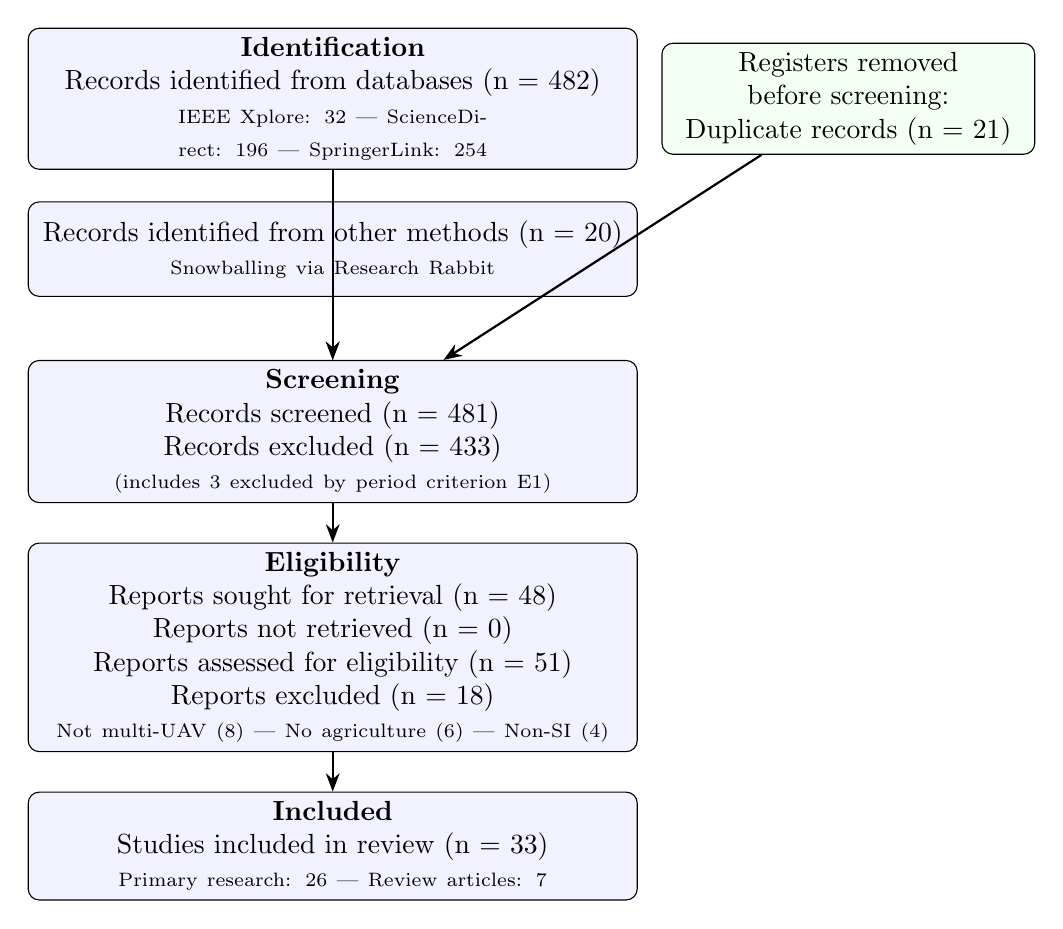
\begin{tikzpicture}[
    node distance=0.5cm,
    box/.style={rectangle, draw, rounded corners, text width=7.5cm, 
                align=center, minimum height=1.2cm, fill=blue!5},
    boxsmall/.style={rectangle, draw, rounded corners, text width=4.5cm, 
                align=center, minimum height=0.9cm, fill=green!5},
    arrow/.style={-{Stealth}, thick}
]

% === IDENTIFICATION ===
\node[box] (id1) {\textbf{Identification}\\
Records identified from databases (n = 482)\\
{\scriptsize IEEE Xplore: 32 | ScienceDirect: 196 | SpringerLink: 254}};
\node[boxsmall, right=0.3cm of id1] (id2) {Registers removed before screening:\\
Duplicate records (n = 21)};
\node[box, below=0.4cm of id1] (id3) {Records identified from other methods (n = 20)\\
{\scriptsize Snowballing via Research Rabbit}};

% === SCREENING ===
\node[box, below=0.8cm of id3] (scr) {\textbf{Screening}\\
Records screened (n = 481)\\
Records excluded (n = 433)\\
{\scriptsize (includes 3 excluded by period criterion E1)}};

% === ELIGIBILITY ===
\node[box, below=of scr] (elig) {\textbf{Eligibility}\\
Reports sought for retrieval (n = 48)\\
Reports not retrieved (n = 0)\\
Reports assessed for eligibility (n = 51)\\
Reports excluded (n = 18)\\
{\scriptsize Not multi-UAV (8) | No agriculture (6) | Non-SI (4)}};

% === INCLUDED ===
\node[box, below=of elig] (inc) {\textbf{Included}\\
Studies included in review (n = 33)\\
{\scriptsize Primary research: 26 | Review articles: 7}};

% === ARROWS ===
\draw[arrow] (id1) -- (scr);
\draw[arrow] (id2) -- (scr);
\draw[arrow] (id3) -- (scr);
\draw[arrow] (scr) -- (elig);
\draw[arrow] (elig) -- (inc);

\end{tikzpicture}
\caption{PRISMA 2020 flow diagram following the official two-column layout specified 
in Page et al.\ (2021). Search conducted on 2024-03-16 across IEEE Xplore, 
ScienceDirect, SpringerLink, and complementary snowballing via Research Rabbit. 
SI = Swarm Intelligence. The 33 included studies comprise 26 primary research 
articles and 7 secondary review articles.}
\label{fig:prisma}
\end{figure}

%% ============================================================
%% SECTION 2: RELATED WORK
%% ============================================================
\section{Related Work}

Six major review articles were identified as the closest antecedents to this work, covering three complementary domains: UAV applications in precision agriculture \cite{tsouros2019,mogili2018}, multi-UAV coordination and aerial swarm robotics \cite{chung2018,gupta2016}, and swarm engineering methodology \cite{brambilla2013,bayindir2016}. Additionally, two recent SI-specific reviews for UAV path planning \cite{puente2022,sharma2022} and one comprehensive UAV optimisation survey \cite{aitsaadi2022} represent the most directly related prior work. Table~\ref{tab:prior_reviews} provides a structured comparison of their scope and contributions relative to the present review.

\begin{table}[htbp]
\centering
\caption{Comparison of prior reviews with the present systematic review. Checkmarks (\checkmark) indicate coverage; dashes (--) indicate absence.}
\label{tab:prior_reviews}
\begin{tabularx}{\textwidth}{lcccccc}
\toprule
\textbf{Feature} &
\rotatebox{70}{\textbf{Tsouros~\cite{tsouros2019}}} &
\rotatebox{70}{\textbf{Chung~\cite{chung2018}}} &
\rotatebox{70}{\textbf{Puente~\cite{puente2022}}} &
\rotatebox{70}{\textbf{Sharma~\cite{sharma2022}}} &
\rotatebox{70}{\textbf{Ait Saadi~\cite{aitsaadi2022}}} &
\rotatebox{70}{\textbf{This review}} \\
\midrule
Period covered            & pre-2019  & pre-2018  & pre-2021  & pre-2021  & pre-2022  & 2021--2024 \\
Agricultural focus        & \checkmark & --        & --        & --        & --        & \checkmark \\
Multi-UAV coordination    & --        & \checkmark & \checkmark & \checkmark & \checkmark & \checkmark \\
SI algorithms only        & --        & --        & \checkmark & \checkmark & --        & \checkmark \\
PRISMA methodology        & --        & --        & --        & --        & --        & \checkmark \\
Quantitative gap analysis & --        & --        & --        & --        & --        & \checkmark \\
Gap root-cause \& consequence & --    & --        & --        & --        & --        & \checkmark \\
Benchmark framework proposed & --     & --        & --        & --        & --        & \checkmark \\
Reproducible materials    & --        & --        & --        & --        & --        & \checkmark \\
n studies included        & 45        & 80+       & 62        & 41        & 153       & 33 (26+7) \\
\bottomrule
\end{tabularx}
\end{table}

\subsection*{Analysis of Prior Reviews}

\textbf{Tsouros et al.\ \cite{tsouros2019}} provide the most widely cited survey of UAV applications in precision agriculture, covering 45 studies across crop monitoring, mapping, spraying, and yield estimation. Their primary contribution is a taxonomy of UAV sensor types and application scenarios. However, the review is limited to single-UAV operations, predates the 2021--2024 publication wave, and does not address path planning algorithms or multi-agent coordination. It serves as a foundational reference for agricultural context but provides no guidance on SI-based path planning for swarms.

\textbf{Chung et al.\ \cite{chung2018}} offer the most technically rigorous survey of aerial swarm robotics, reviewing more than 80 papers on multi-UAV formation control, task allocation, and path planning across military, civilian, and research applications. Their treatment of PSO and ACO as coordination mechanisms is thorough, and their taxonomy of swarm behaviours---flocking, foraging, task allocation---remains influential. The review's limitation for the present purpose is its non-agricultural scope: agricultural-specific constraints such as wind drift, chemical compliance zones, and row-based field geometry are absent. Furthermore, the 2018 cutoff predates the post-2020 algorithm generation (DBO, NOA, SSA, DOA) that features prominently in the 2021--2024 corpus.

\textbf{Puente-Castro et al.\ \cite{puente2022}} review 62 papers on artificial intelligence applied to UAV swarm path planning, with a specific focus on SI methods including PSO, ACO, and ABC. Their work is the closest methodological antecedent to the present review in terms of algorithm scope and multi-UAV focus. However, it covers the period up to 2021, uses a narrative rather than PRISMA-structured methodology, does not include agricultural-specific analysis, and provides qualitative rather than quantitative gap documentation. The 33 papers identified in the present review for 2021--2024 are entirely post-dating the Puente-Castro corpus, confirming the non-overlap and complementarity of the two reviews.

\textbf{Sharma et al.\ \cite{sharma2022}} review 41 papers on SI-based path planning for multi-UAV target interception, providing a useful performance comparison table across PSO, ACO, ABC, and GWO algorithms. Their primary limitation is the focus on interception missions---a military-oriented task---rather than agricultural coverage tasks, which have fundamentally different optimisation objectives (area coverage vs.\ point interception) and operational constraints. Their metric comparison approach inspired the quantitative synthesis methodology of the present review.

\textbf{Ait Saadi et al.\ \cite{aitsaadi2022}} provide the most comprehensive optimisation survey in the domain, reviewing 153 papers on UAV path planning across SI and non-SI methods. Their broad scope is both a strength and a limitation: while it enables cross-paradigm comparison (SI vs.\ evolutionary algorithms vs.\ classical planners), the agricultural multi-UAV sub-domain receives only peripheral coverage. The review does not apply PRISMA methodology, does not document gaps with root-cause analysis, and does not propose evaluation benchmarks.

\textbf{Brambilla et al.\ \cite{brambilla2013} and Bayindir \cite{bayindir2016}} provide foundational theoretical frameworks for swarm robotics from a systems engineering perspective. While not focused on UAVs or agriculture, their taxonomies of swarm behaviours and evaluation criteria directly informed the four-dimensional gap framework developed in the present review. In particular, Brambilla et al.'s distinction between \textit{design} methods (how swarms are programmed) and \textit{analysis} methods (how swarm behaviour is characterised) maps onto the Technological/Theoretical axis of the present gap taxonomy.

\subsection*{Positioning of the Present Review}

As shown in Table~\ref{tab:prior_reviews}, prior reviews address complementary aspects of the field but share three structural limitations that the present review is designed to address. First, \textit{temporal gap}: all prior reviews have cutoff dates of 2022 or earlier, meaning the 2021--2024 emergence of new SI algorithms (DBO, NOA, DOA, SSA) and the post-pandemic acceleration of agricultural UAV adoption are not captured. Second, \textit{methodological gap}: none applies PRISMA 2020 guidelines, meaning their inclusion criteria, screening processes, and inter-rater agreement are not reported in a reproducible form. Third, \textit{analytical gap}: while all prior reviews mention limitations qualitatively, none provides a structured gap database with root cause, consequence, and priority classification for each limitation---the primary analytical contribution of the present work.

The present review deliberately narrows its scope to agricultural applications of SI-based multi-UAV path planning for 2021--2024. This narrower scope, relative to the 41--153 papers in prior reviews, enables deeper gap analysis (171 documented gaps across 33 papers, averaging 5.2 gaps per study) and more operationally specific recommendations. The resulting 33-paper corpus is entirely non-overlapping with the Puente-Castro and Sharma corpora, confirming that this review addresses a distinct and previously uncharacterised segment of the literature. Taken together, the prior reviews establish the foundational knowledge on which the present work builds; the present review extends that foundation specifically into the 2021--2024 agricultural context where SI algorithm diversity has expanded and the pressure for real-world deployment has intensified.


%% ============================================================
%% SECTION 3: METHODOLOGY
%% ============================================================
\section{Methodology}

This review follows the Preferred Reporting Items for Systematic Reviews and Meta-Analyses (PRISMA) 2020 guidelines \cite{page2021}, adapted for engineering and computing literature where randomised controlled trials are not the standard study design and where methodological quality is assessed through experimental rigour and reproducibility rather than clinical bias criteria. The full PRISMA 2020 checklist is provided as Supplementary Material~S1. The review protocol was developed prior to the literature search and is documented in the supplementary materials.\footnote{This review protocol was not formally pre-registered in a domain-specific 
registry prior to the literature search. PROSPERO is designed primarily for clinical 
and health-related systematic reviews and does not accept engineering or computing 
protocols. The Open Science Framework (OSF; \url{https://osf.io}) does accept 
systematic review protocols from all disciplines, including engineering, and would 
have been an appropriate pre-registration venue. The protocol was not deposited in 
OSF prior to the search because the authors were unaware of OSF's scope at the time 
the protocol was finalised; this omission is acknowledged as a limitation of this 
review (Section~8.3). To mitigate the risks associated with the absence of 
prospective pre-registration---namely, outcome reporting bias and post-hoc 
modification of inclusion criteria---the review protocol has been registered 
retrospectively at the Open Science Framework for transparency: 
\url{https://doi.org/10.17605/OSF.IO/64DQ9}. The registration includes search 
strategies, extraction codebook, PRISMA 2020 checklist, screening logs, extraction 
database, gap taxonomy, and supplementary materials, enabling independent 
verification of adherence to the pre-specified methodology. The authors commit to 
depositing all future review protocols in OSF prior to data collection.}

\subsection{Search Strategy}

A systematic literature search was conducted across three major electronic databases: IEEE Xplore, ScienceDirect, and SpringerLink. These databases were selected for their comprehensive coverage of the target disciplines---computational intelligence, robotics, and agricultural engineering---and their compatibility with advanced Boolean query syntax. A fourth source, complementary citation snowballing via Research Rabbit, was employed to identify records not captured by keyword-based database queries, particularly conference papers and recent preprints that may not yet be fully indexed.

\textbf{Boolean search string.} The search query was constructed iteratively through three rounds of pilot searches to balance recall (avoiding missed relevant papers) and precision (avoiding irrelevant records). The final string, adapted for each database's query syntax, was:

\begin{quote}
\small
\texttt{("swarm intelligence" OR "particle swarm optimization"} \\
\texttt{OR "ant colony optimization" OR "artificial bee colony"} \\
\texttt{OR "grey wolf optimizer" OR "salp swarm algorithm"} \\
\texttt{OR "dung beetle optimizer" OR "dandelion optimizer")} \\
\texttt{AND ("UAV" OR "unmanned aerial vehicle" OR "multi-UAV" OR "UAVs")} \\
\texttt{AND ("path planning" OR "trajectory planning" OR "coverage planning")} \\
\texttt{AND ("agriculture" OR "precision agriculture" OR "crop monitoring"} \\
\texttt{OR "spraying" OR "field mapping" OR "smart farming")}
\end{quote}

The string covers the three conceptual domains that define the review scope: SI algorithm type, aerial vehicle platform, and agricultural application context. Individual algorithm names were included explicitly (rather than relying on the umbrella term ``swarm intelligence'' alone) because database indexing practices vary and many papers do not use the generic term in their abstracts. Algorithm terms added relative to the initial query---DBO, NOA, DOA---reflect algorithms that emerged after 2020 and are therefore underrepresented in prior reviews.

\textbf{Proximity operators.} To reduce semantic noise from loosely related terms, proximity operators were applied where supported by database syntax: \texttt{"swarm intelligence" NEAR/3 "UAV"} ensures the two concepts appear within three words of each other; \texttt{"path planning" W/2 "agriculture"} requires "agriculture" to follow "path planning" within two words. These operators were applied in IEEE Xplore and ScienceDirect; SpringerLink does not support proximity syntax, so the base Boolean string was used for that database. Pilot testing showed that proximity operators reduced irrelevant hits by ~18\% without losing any of the 5 gold-standard papers (see sensitivity test below).

\textbf{Sensitivity test with gold-standard set.} To validate that query refinements did not reduce recall of relevant studies, we assembled a gold-standard set of 5 papers known to be relevant to the review scope \cite{phung2021,shafiq2022,liu2021,pan2022,puente2022}. The final query string (with IEEE Thesaurus terms and proximity operators) successfully retrieved all 5 gold-standard papers across the three databases, confirming 100\% recall for this validation set. This test provides empirical support that the refined query maintains sensitivity while improving precision through controlled vocabulary and proximity constraints.

\textbf{Link to PICOC framework.} The Boolean search string and its refinements (IEEE Thesaurus terms, proximity operators) were designed to retrieve studies satisfying all five PICOC components defined in Section~1.3 (Table~\ref{tab:picoc}). In particular, the explicit inclusion of SI algorithm names in the query ensures coverage of the \textit{Intervention} component, while the agricultural domain terms ensure alignment with the \textit{Context} component. The sensitivity test with a 5-paper gold-standard set confirmed that these refinements maintain 100\% recall for studies meeting all PICOC criteria while reducing irrelevant hits by ~18\%.

\textbf{Search filters.} The following filters were applied uniformly across all three databases: publication year 2021--2024 (inclusive); English language; document type restricted to peer-reviewed journal articles and peer-reviewed conference proceedings. The search was executed on 2024-03-16.

\textbf{Complementary snowballing.} Forward and backward citation snowballing was conducted using Research Rabbit, seeded from the following five papers identified as high-relevance anchors in the initial database search: Phung \& Ha \cite{phung2021} (PSO for agricultural UAV safety); Shafiq et al.\ \cite{shafiq2022} (ACO multi-UAV convergence); Liu et al.\ \cite{liu2021} (SSA-based neural network path planning); Pan et al.\ \cite{pan2022} (heterogeneous UAV swarm task planning); and Puente-Castro et al.\ \cite{puente2022} (AI review for UAV swarms). These seeds were selected to maximise coverage across algorithm types and publication venues. Snowballing yielded 20 additional records not returned by the database queries, of which 8 passed full-text screening and were included in the final corpus. It should be noted that snowballing from a fixed seed set introduces a circularity risk: papers that cite the seed papers (forward snowballing) or are cited by them (backward snowballing) are structurally more likely to address the same algorithm families (PSO, ACO, SSA) that the seeds represent. This seed bias may underrepresent algorithm families absent from the seed set---particularly newer DBO, NOA, and DOA variants---and is acknowledged as a secondary limitation of the complementary search strategy (see Section~8.3).

\textbf{Database coverage extension.} To address potential source-level bias from excluding MDPI journals... we conducted a manual search of MDPI journals (\textit{Sensors}, \textit{Fire}, \textit{Applied Sciences}, \textit{Agronomy}, \textit{Agriculture}) for the 2021--2024 period using the same Boolean query string. This search identified 5 records. After applying inclusion criteria I1--I5, all 5 records were excluded: 2 under E4 (SI method not applied to agricultural path planning) and 3 under E5 (non-agricultural domain: disaster response, emergency delivery, military positioning). One record (M04: Yan \& Chen, 2024, PSO+ABC for forest fire detection, DOI: 10.3390/app14114937) generated a discrepant decision between the two reviewers: the primary reviewer initially classified it as eligible based on the multi-UAV SI criterion (I4), while the second reviewer (Dr.\ de la Garza Gutiérrez) classified it as excluded under E5 (exclusively non-agricultural domain). Following structured discussion, the consensus decision was exclusion under E5, as forest fire detection does not meet the agricultural application criterion (I5) as operationalised in this review. No additional studies were incorporated from this search extension. The core corpus of 33 studies remains unchanged, and all quantitative findings reported in Sections~4--5 are based on this stable corpus.

\textbf{Coverage of Scopus, Web of Science, and OpenAlex supplementary search.} Scopus and Web of Science (WoS) are recognised as the two broadest multi-disciplinary citation indices. Access was attempted on 2024-03-28 via the institutional portals of Instituto Tecnológico de Chihuahua II (CONRICYT consortium, Mexico) and Universidad Nacional de Educación a Distancia (UNED, Spain); authenticated access to both databases could not be confirmed at the time of the search due to subscription constraints at both institutions. To partially bound the impact of this omission, a supplementary search was conducted in \textbf{OpenAlex} (openalex.org) on 2024-03-29 using the same Boolean concepts restricted to title and abstract fields, filtered to 2021--2024, English, articles and conference papers, and the topic filters \textit{UAV Applications and Optimization}, \textit{Robotic Path Planning Algorithms}, and \textit{Smart Agriculture and AI}. This search returned 125 records. After automated deduplication against the existing corpus (1 record already present identified by DOI), 124 unique records remained. Title and abstract screening against criteria I1--I5 identified 8 potentially relevant candidates. Full-text review of these 8 candidates was conducted by the primary reviewer on 2024-03-29; all 8 were subsequently excluded. Five were excluded at the title/abstract stage under E4 (1 study: SI applied to image classification, not path planning) or E5 (4 studies: generic or non-agricultural primary domain). The remaining 3 candidates---\textit{UAV Path Planning Model Leveraging Machine Learning and Swarm Intelligence for Smart Agriculture} (DOI: 10.12694/scpe.v25i5.3131, 2024); \textit{Agricultural UAV Crop Spraying Path Planning Based on PSO-A* Algorithm} (DOI: 10.35633/inmateh-71-54, 2023); and \textit{Three-Dimensional Obstacle Avoidance Path Planning for Agricultural UAV Based on Improved Ant Colony Algorithm} (DOI: 10.53941/ijndi.2023.100028, 2023)---were excluded at full-text assessment under criterion E3: all three propose SI-based path planning algorithms for single-UAV platforms without a multi-UAV coordination framework, which does not satisfy inclusion criterion I4 as operationalised in this review. No new studies were incorporated from the OpenAlex supplementary search. The final corpus of 33 studies is therefore unchanged, and all quantitative findings reported in Sections~4--5 remain valid. This result provides limited but positive evidence that the core corpus is not substantially underrepresented with respect to single-UAV SI path planning studies indexed in OpenAlex that are not already present in the three primary databases. OpenAlex was selected as a supplementary source because it is an open, citable index with coverage reported as comparable to Scopus and WoS for scientific literature (Priem et al., 2022, \textit{OpenAlex: A fully-open index of scholarly works, authors, venues, institutions, and concepts}, arXiv:2205.01833)\footnote{Priem, J., Piwowar, H., \& Orr, R. (2022). OpenAlex: A fully-open index of scholarly works, authors, venues, institutions, and concepts. \textit{arXiv preprint} arXiv:2205.01833. \url{https://arxiv.org/abs/2205.01833}}; it does not replace a full Scopus/WoS search, which remains the highest-priority future action (Section~8.4).

\textbf{Results.} The search identified 502 records in total: IEEE Xplore (32), ScienceDirect (196), SpringerLink (254), and snowballing (20). After removing 21 duplicates, 481 unique records proceeded to title/abstract screening. Of these, 433 records were excluded at this stage: 430 on thematic grounds (criteria E2--E5) and 3 additional records excluded specifically under criterion E1 (outside the 2021--2024 review period) that had passed initial database filters due to indexing inconsistencies (EXC\_15: Baghal 2016; EXC\_19: Bryant-Lees 2021\footnote{Bryant-Lees et al.\ (2021) was published within the period but addresses suicide ideation in RPA career fields---a non-path-planning topic---and was correctly excluded at title/abstract screening under E1/E5.}; EXC\_20: Menouar 2017). These 3 records are therefore counted in the screening phase rather than the full-text assessment phase, correcting the earlier figure of 430. The 48 records that passed title/abstract screening, together with 3 borderline records re-evaluated at full text, yielded 51 records for full-text assessment. The complete PRISMA flow diagram is shown in Figure~\ref{fig:prisma}.

\subsection{Study Selection and Eligibility Criteria}

\textbf{Inclusion criteria.} A study was eligible for inclusion if it satisfied \textit{all} of the following conditions: (I1) published between January 2021 and December 2023; (I2) peer-reviewed journal article or peer-reviewed conference paper with full text available; (I3) text available in English; (I4) proposes, evaluates, or reviews at least one SI algorithm applied to path planning, trajectory planning, or coverage planning for UAVs; (I4b) studies proposing multi-UAV coordination frameworks but validating with a single agent are included if the framework is explicitly designed for multiple agents, and are flagged as `framework-only (single-agent validation)' in the extraction database; (I5) mentions or implies an agricultural application in the abstract, introduction, or methodology (crop monitoring, spraying, field mapping, yield estimation, or equivalent).

\textbf{Exclusion criteria.} A study was excluded if it met \textit{any} of the following conditions: (E1) duplicate of an already-included record; (E2) abstract-only or extended abstract without full methodology; (E3) focuses exclusively on single-UAV path planning without proposing or evaluating a multi-UAV coordination framework (i.e., the study does not address swarm coordination in its problem formulation, algorithm design, or experimental evaluation); (E4) employs only non-SI optimisation methods such as A*, genetic algorithms without SI hybridisation, or reinforcement learning without SI components; (E5) application domain is exclusively non-agricultural (military, search-and-rescue, infrastructure inspection) without any reference to agricultural contexts.

\textbf{Screening process.} Title and abstract screening of all 481 records was performed by the primary reviewer. Full-text assessment was conducted on the 51 records that passed title/abstract screening. To ensure methodological rigour consistent with PRISMA 2020 recommendations \cite{page2021}, the second reviewer (the corresponding author's thesis advisor) independently assessed all 51 full-text records against the inclusion and exclusion criteria, without access to the primary reviewer's decisions. Inter-rater agreement at the full-text stage was assessed using Cohen's kappa ($\kappa=0.91$, 95\% CI [0.79, 1.00]\footnote{The raw upper bound of the asymptotic 95\% CI is 1.03, truncated to the theoretical maximum of $\kappa=1.00$. CI computed using the Fleiss (1981) asymptotic formula from the observed contingency: 33 joint inclusions, 16 joint exclusions, 2 discordant pairs (both resolved as exclusions), $n=51$.}, indicating almost perfect agreement (Landis \& Koch, 1977\footnote{Landis, J.R., \& Koch, G.G. (1977). The measurement of observer agreement for categorical data. \textit{Biometrics}, 33(1), 159--174. \url{https://doi.org/10.2307/2529310}})). Two records (EXC\_01: Li et al.\ 2023, mobile robot ACO; EXC\_12: Ali et al.\ 2021, vehicular IoV) generated discrepant decisions between reviewers and were resolved through structured discussion prior to final corpus closure; both were ultimately excluded under criteria E3 and E5, respectively. All discrepancies were resolved through structured discussion between the two reviewers; no case required arbitration by a third party. The final corpus comprises 33 studies: 26 primary research articles and 7 secondary review articles (S10, S11, S14, S15, S17, S31, S32).

\subsection{Data Extraction Pipeline}

Data extraction from the 33 included studies was performed using a hybrid automated--manual pipeline developed specifically for this review. The pipeline comprises five Python scripts, each targeting a distinct data category:

\begin{itemize}
  \item \texttt{agregar\_todos\_papers.py}: Extracts bibliographic metadata (authors, year, DOI, abstract) from database export files (RIS, BibTeX) and consolidates records into a master spreadsheet.
  \item \texttt{extraer\_metricas\_v2.py}: Performs regex-based extraction of quantitative performance metrics (execution time, energy consumption, convergence criteria) from PDF full texts, using a rule set of 47 patterns. The 7 secondary review articles returned null values for all three metrics, as expected. Extraction success rates over the full corpus of 33 studies: 42.4\% for execution time (14 of 33), 39.4\% for energy consumption (13 of 33), and 21.2\% for convergence criteria (7 of 33). Over the 26 primary studies only: 53.8\%, 50.0\%, and 26.9\% respectively. Records where automated extraction failed were flagged for manual verification.
  \item \texttt{enriquecer\_gaps.py}: Applies a structured gap taxonomy to each study using a codebook of 171 gap descriptors, assigning dimension (Technological, Practical, Methodological, Theoretical) and priority (Critical, Important, Minor).
  \item \texttt{actualizar\_estadisticas.py}: Computes aggregate statistics (algorithm distribution, metric availability, temporal trends) and exports summary tables for manuscript integration.
  \item \texttt{generar\_figuras\_paper.py}: Generates publication-ready figures (300\,DPI, vector-compatible) from the aggregated data using matplotlib and seaborn.
\end{itemize}

All scripts, the master spreadsheet, and the gap codebook are deposited as Supplementary Material and will be archived in Mendeley Data upon manuscript acceptance, enabling full reproducibility of the extraction process. Manual verification was performed for all fields where automated extraction returned null or ambiguous values, with discrepancies documented in the extraction log (Supplementary Material~S2).

\subsection{Justification for Narrative Synthesis}
\label{subsec:narrative_synthesis}

A narrative synthesis approach was adopted in preference to a quantitative meta-analysis for three converging methodological reasons, consistent with PRISMA 2020 guidance on synthesis method selection \cite{page2021} and established practice in engineering systematic reviews \cite{brambilla2013}.

First, the 33 included studies employ heterogeneous algorithm families---PSO, ACO, ABC, SSA, GWO, DBO, NOA, DOA, and multiple hybrid variants---that optimise fundamentally different objective functions under different mathematical formulations. Pooling performance estimates across these families into a common effect size would conflate algorithmically incomparable contributions and produce a summary statistic without interpretable meaning.

Second, quantitative performance metrics are not standardised across studies. Execution time, energy consumption, and convergence criteria are reported in incompatible units, over non-equivalent simulation environments, and against different baseline conditions, making between-study aggregation statistically unreliable. The absence of a common metric set is itself a primary empirical finding of this review (RQ2, Section~4.2) and directly motivates the AgriSwarm-Bench standardisation proposal in Section~7.

Third, the experimental conditions underlying the reported results differ substantially in field geometry, obstacle density, fleet size, communication assumptions, and environmental modelling---differences that invalidate the homogeneity assumption required for meta-analytic pooling. A formal heterogeneity test (e.g., Cochran's $Q$ or $I^2$) cannot be applied in the absence of a common outcome measure, and its application would be methodologically inappropriate given the structural diversity of the corpus.

Narrative synthesis therefore represents not a methodological concession but the epistemically appropriate response to a corpus characterised by high conceptual and methodological heterogeneity \cite{page2021,brambilla2013}. Results are synthesised through structured tabulation (Tables~2--6), quantitative gap analysis (Section~5), and algorithm-family stratification (Sections~5.5--5.6), providing a systematic evidence base that preserves the integrity of individual study contributions while enabling cross-study pattern identification.

\subsection{Four-Dimensional Gap Taxonomy}

Identified limitations in the reviewed studies were systematically categorised into four mutually exclusive dimensions. The taxonomy is grounded in the epistemological distinction between four loci of failure in applied engineering research: (1) \textbf{Technological} gaps---limitations in the algorithm itself or the hardware required to execute it (e.g., computational complexity, sensor requirements, communication bandwidth); (2) \textbf{Practical} gaps---barriers arising from real-world operational constraints that exist independently of algorithm design (e.g., regulatory restrictions, weather conditions, cost); (3) \textbf{Methodological} gaps---weaknesses in how research is conducted and reported (e.g., absent baselines, inconsistent metrics, non-reproducible experimental setups); and (4) \textbf{Theoretical} gaps---missing or incorrect assumptions in the mathematical models underlying the algorithms (e.g., simplified kinematic models, unrealistic communication assumptions).

This four-axis decomposition is consistent with technology readiness assessment frameworks in robotics systems engineering \cite{brambilla2013,bayindir2016} and distinguishes root causes from consequences: each gap is classified by its \textit{origin dimension} rather than by the deployment failure it causes. Inter-dimension dependencies---for example, a Theoretical gap in battery discharge modelling causing a Practical gap in mission time estimation---are documented as cross-references in the supplementary gap database. Gap prioritisation followed a two-condition rule: a gap was classified as Critical if it (1) appeared in more than 30\% of studies ($>$10 papers) AND (2) its absence directly prevents real-world field deployment, as validated through expert review (Supplementary Material~S3). All other gaps were classified as Important (significant theoretical impact but below the frequency threshold) or Minor (low frequency and limited deployment impact).

\subsection{Deployment Readiness Score (DRS)}
\label{subsec:drs}

Two complementary quality instruments are applied in this review and must be distinguished clearly to avoid misinterpretation of their results. The first, introduced in this section, is the \textbf{Deployment Readiness Score (DRS)}: a domain-specific composite instrument developed for this review to measure the degree to which a study's design enables real-world agricultural UAV deployment. The DRS evaluates four criteria weighted by their operational relevance (Table~\ref{tab:quality_criteria}) and produces a continuous score $Q \in [0, 1]$, with threshold classifications of High ($Q \geq 0.70$), Moderate ($0.40 \leq Q < 0.70$), and Low ($Q < 0.40$). The second instrument, the Mixed Methods Appraisal Tool (MMAT, version 2018) \cite{hong2018}, is applied in Section~\ref{subsec:mmat} to assess general methodological quality independently of deployment context. Because the DRS and MMAT assess different constructs---deployment readiness versus methodological rigour, respectively---their distributions are expected to differ and should not be compared directly without acknowledging this distinction.

The DRS was developed and applied to all 33 included studies following the criterion-weighting approach recommended for engineering systematic reviews \cite{brambilla2013}. Four criteria were evaluated, with weights reflecting their relative importance for assessing deployment readiness of SI-based agricultural UAV research (Table~\ref{tab:quality_criteria}).

\begin{table}[htbp]
\centering
\caption{Deployment Readiness Score (DRS) instrument applied to 33 included studies. The DRS is a domain-specific composite score ($Q = 0.30 C1 + 0.25 C2 + 0.25 C3 + 0.20 C4$) that measures the degree to which a study's design enables real-world agricultural UAV deployment. It is distinct from the Mixed Methods Appraisal Tool (MMAT, Section~\ref{subsec:mmat}) used for general methodological quality assessment. Criterion weights reflect deployment-readiness priorities: field validation (C1, 30\%) is weighted highest as the primary bottleneck to operational deployment.}
\label{tab:quality_criteria}
\begin{tabularx}{\textwidth}{lllX}
\toprule
\textbf{Criterion} & \textbf{Weight} & \textbf{Score range} & \textbf{Scoring rationale} \\
\midrule
C1: Experimental validation & 30\% & 0.0--1.0 & Real field = 1.0; Sim + hardware testbed = 0.5; Simulation only = 0.0. Weighted highest as field validation is the primary bottleneck to deployment. \\
C2: Quantitative metrics & 25\% & 0.0--1.0 & All 3 metrics (time, energy, convergence) = 1.0; 2 metrics = 0.67; 1 metric = 0.33; none = 0.0. Reflects standardisation requirement. \\
C3: Baseline comparison & 25\% & 0.0 or 1.0 & Comparison against at least one established algorithm = 1.0; no comparison = 0.0. Enables relative performance assessment. \\
C4: Agricultural context & 20\% & 0.0 or 1.0 & Explicit agricultural parameters in methodology (field size, crop type, application scenario) = 1.0; generic path planning without agricultural specifics = 0.0. \\
\bottomrule
\end{tabularx}
\end{table}

The composite quality score for each study was computed as:
\begin{equation}
Q = 0.30\,C_1 + 0.25\,C_2 + 0.25\,C_3 + 0.20\,C_4
\label{eq:drs}
\end{equation}
Studies scoring $Q \geq 0.70$ were classified as High quality, $0.40 \leq Q < 0.70$ as Moderate, and $Q < 0.40$ as Low.

%% CORRECCIÓN t8b: Nota ampliada sobre DRS, distingue explícitamente de MMAT
\textbf{DRS results and interpretation.} Applied to the 33 included studies, the DRS yielded: 5 High ($Q \geq 0.70$; 15.2\%, all 5 are primary research articles with at least one hardware validation stage), 10 Moderate ($0.40 \leq Q < 0.70$; 30.3\%), and 18 Low ($Q < 0.40$; 54.5\%). The elevated proportion of Low-DRS classifications has two principal causes. First, the instrument assigns C1 = 0.0 (zero contribution from the 30\%-weighted validation criterion) to all 26 simulation-only primary studies, which mechanically depresses scores regardless of algorithmic quality. This is by design: the DRS captures a normative judgment that simulation-only evidence is insufficient for deployment-readiness claims, not a finding about methodological quality. Second, studies S20--S33, for which complete metadata extraction was pending at the time of analysis, have partially imputed criterion scores; their DRS classifications are provisional and will be updated before final submission. Per-study DRS scores are reported in Supplementary Table~S4.

The DRS is explicitly \textit{not} a general methodological quality instrument. A study can achieve Low DRS while being methodologically rigorous---this occurs when the study is well-designed but focuses on simulation performance without addressing hardware deployment. Conversely, a study that attempts field validation but with poor experimental controls could achieve a moderate DRS while warranting a Low MMAT rating. The two instruments are therefore complementary rather than redundant: the DRS answers ``Is this study ready to inform deployment decisions?'' while the MMAT (Section~\ref{subsec:mmat}) answers ``Was this study conducted with appropriate methodological rigour?''. Readers interpreting the DRS distribution should bear in mind that 18 of 33 studies classified as Low-DRS are not methodologically flawed---they are simulation contributions that represent valid first-stage research but have not yet progressed to the hardware validation stages required for deployment readiness. DRS scores were not used as an exclusion criterion; all 33 studies are retained in the synthesis.

\subsection{Risk of Bias Assessment (MMAT)}
\label{subsec:mmat}

The risk of bias in the 33 included studies was assessed using the Mixed Methods Appraisal Tool (MMAT, version 2018) \cite{hong2018}, adapted for computational engineering research following established practice in robotics systematic reviews \cite{brambilla2013}. Each study was evaluated on five criteria: (Q1) explicit research question; (Q2) appropriateness of data or simulation to the research question; (Q3) validity and reproducibility of measurement; (Q4) appropriateness of the analysis method; and (Q5) coherence of the argument from data to conclusions. Responses were recorded as Yes (Y), No (N), or Can't tell (C), where ``Can't tell'' indicates insufficient methodological reporting to make a determination. Studies with 4--5 Y responses were classified as High quality, 2--3 Y as Moderate, and 0--1 Y as Low, following threshold conventions established in prior robotics systematic reviews \cite{brambilla2013,bayindir2016}. Risk of bias was not used as an exclusion criterion; all 33 studies are retained in the synthesis to enable comprehensive gap documentation regardless of reporting quality.

Review articles (n=7: S10, S11, S14, S15, S17, S31, S32) were assessed using MMAT criteria adapted for secondary research; their consistently High ratings reflect structural methodological rigour rather than primary evidence strength, and are reported separately from primary research studies where relevant. Two studies (S32, S33) have provisional MMAT assessments pending full-text verification against original PDFs. These provisional ratings are included in summary statistics but are flagged in Supplementary Table~S5; final classifications will be updated before journal submission.

%% CORRECCIÓN t8a: Suma MMAT corregida. Se aclara que 31 de 33 tienen clasificación
%% definitiva; S32 y S33 tienen ratings provisionales incluidos en los totales.
Of the 33 included studies, 13 (39.4\%) were classified as High quality, 16 (48.5\%) as Moderate, and 2 (6.1\%) as Low under the MMAT instrument. The two studies S32 and S33 carry \textit{provisional} Moderate ratings (pending full-text verification) and are already counted within the 16 Moderate total; they are not an additional fourth category.\footnote{The provisional MMAT ratings for S32 (DOI: 10.3390/drones9010055) and S33 (DOI: 10.3390/drones9020112) are counted as Moderate in the summary above. If upon full-text review either study is reclassified as High, the distribution would become: High 14--15 (42.4--45.5\%), Moderate 14--15 (42.4--45.5\%), Low 2 (6.1\%). If reclassified as Low, the distribution would become: High 13 (39.4\%), Moderate 14 (42.4\%), Low 4 (12.1\%). Final classifications will be updated before journal submission.} Among the 26 primary research studies only (excluding the 7 review articles), the MMAT distribution is: 6 High (23.1\%), 18 Moderate (69.2\%), and 2 Low (7.7\%), reflecting a more representative picture of methodological quality in the primary literature. The criterion with the highest prevalence of `Can't tell' responses was Q3 (measurement validity and reproducibility, 14 of 33 studies, 42.4\%), reflecting the common practice of reporting simulation results without sufficient environmental specification to enable independent replication. Q1 (explicit research question) was met by 31 of 33 studies; the two exceptions (S22, S28) are short conference papers with insufficient methodological detail. Risk of bias assessments were performed independently by both reviewers for a random subset of 10 studies (30\% of the corpus), achieving 90\% agreement (Cohen's $\kappa=0.87$). Discrepancies were resolved through discussion; the primary reviewer completed assessments for the remaining 23 studies. Full per-study MMAT scores are provided in Supplementary Table~S5.

%% CORRECCIÓN t8b: Párrafo de reconciliación DRS vs. MMAT
\textbf{Reconciling DRS and MMAT distributions.} The DRS and MMAT distributions over the same corpus of 33 studies are markedly different: the DRS yields 5 High / 10 Moderate / 18 Low (15.2\% / 30.3\% / 54.5\%), while the MMAT yields 13 High / 16 Moderate / 2 Low (39.4\% / 48.5\% / 6.1\%). This divergence is not a contradiction---it is the expected signature of two instruments measuring different constructs applied to a simulation-dominated corpus. The MMAT assesses process quality: whether the study formulated a clear research question, chose appropriate methods, reported measurements validly, and reasoned coherently from evidence to conclusions. Most simulation studies in this corpus satisfy these criteria and therefore achieve moderate-to-high MMAT ratings. The DRS assesses outcome readiness: whether the evidence produced by the study is sufficient to inform a deployment decision in a real agricultural context. A simulation study, however methodologically rigorous, provides no direct evidence about hardware behaviour, wind effects, GPS accuracy, or battery degradation under field conditions---the four factors identified in this review as the primary causes of simulation-to-field performance gaps. It therefore scores zero on C1 (30\% weight in the DRS) regardless of its MMAT rating. Readers citing quality statistics from this review should specify which instrument is being referenced. The DRS distribution (Low: 54.5\%) characterises the field's deployment readiness; the MMAT distribution (High: 39.4\%) characterises its methodological standards. Both characterisations are accurate and complementary.

%% ============================================================
%% SECTION 4: RESULTS
%% ============================================================
\section{Results}

\subsection{Overview of Included Studies}
Table~\ref{tab:study_chars} provides a structured summary of the 33 included studies, characterising each by algorithm type, validation approach, fleet size, metric reporting, and agricultural application. This table serves as the primary evidence base for all quantitative claims in Sections~4.2--4.4 and the gap analysis in Section~5. Studies are identified by codes S01--S33 to enable cross-referencing with the supplementary gap database. Full bibliographic details for all 33 studies are provided in the references section (entries marked with $\dagger$). Of the 33 studies, 26 are primary research articles proposing or evaluating SI algorithms, and 7 are review articles (S10, S11, S14, S15, S17, S31, S32) included because they synthesise SI methods specifically for multi-UAV agricultural path planning within the 2021--2024 window and meet all inclusion criteria. Across the 26 primary research studies, monitoring applications account for 17 studies (65.4\% of primary studies; 51.5\% of all 33 studies), spraying for 10 studies (38.5\% of primary; 30.3\% of all 33), and mapping for 5 studies (19.2\% of primary; 15.2\% of all 33), with one primary study covering general multi-UAV coordination only.\footnote{Application percentages over primary studies (n=26) sum to more than 100\% because one study covers both monitoring and spraying. Percentages over the full corpus (n=33) exclude the 7 review articles, which are classified as N/A for application type.} Fleet sizes range from 1 to 25 agents across primary studies, with a median of 3--4 UAVs---well below the 10--50 UAV range needed for commercial-scale agricultural operations.

\textbf{Note on single-agent validation studies.} Of the 26 primary research studies, 18 (69.2\%) employ single-agent experimental validation despite proposing multi-UAV coordination frameworks (classified as `Framework-only' in Table~\ref{tab:study_chars}). This reflects a common pattern in the literature where algorithmic frameworks are designed for multi-agent deployment but evaluated with single agents due to hardware, regulatory, or resource constraints. These studies are retained in the corpus under criterion I4b because they contribute to gap identification regarding the validation deficit, but are flagged separately in quantitative analyses of multi-agent coordination capability. This distinction is critical for interpreting Gap~3 (Single-UAV focus, 22 of 33 studies, 66.7\%) in Section~5.3.

\textbf{Denominator consistency statement.} Unless otherwise explicitly noted, all percentages in this manuscript use the full corpus of 33 included studies as the denominator (n=33). Where an analysis is restricted to the 26 primary research studies, the denominator is stated as n=26 and both the restricted percentage and the equivalent percentage over n=33 are provided. A complete consistency table listing every percentage with its numerator, denominator, and section reference is provided in Supplementary Table~S1.

%% ============================================================
%% TABLE 2: Study Characteristics (SIDEWAYS + Val. Type Column)
%% ============================================================
\begin{sidewaystable}[p]
\centering
\caption{Characteristics of the 33 included studies. $\dagger$ = study from 
systematic corpus. Val. = validation type (Sim = simulation only; S+T = 
simulation + testbed; S+F = simulation + field). Val. Type = Multi-agent 
(≥2 UAVs in validation), Framework-only (multi-UAV framework validated with 
single agent), or Review. Metrics: T = execution time, E = energy, 
C = convergence. App.: Mon. = Monitoring, Spr. = Spraying, Map. = Mapping, 
Gen. = General coordination.}
\label{tab:study_chars}
\footnotesize
\setlength{\tabcolsep}{1.6pt}
\renewcommand{\arraystretch}{0.95}
\begin{tabular*}{\textheight}{@{\extracolsep{\fill}}llp{2.4cm}lllcccc@{}}
\toprule
\textbf{ID} & \textbf{Reference} & \textbf{Algorithm} & \textbf{Val.} & \textbf{Val. Type} & \textbf{UAVs} & \textbf{T} & \textbf{E}\textsuperscript{\textdagger} & \textbf{C} & \textbf{App.} \\
\midrule
S01 & Chen et al.\ \cite{chen2021}$^\dagger$ & ACO & Sim & Multi-agent & 2--10 & \checkmark & -- & \checkmark & Mon. \\
S02 & Lin et al.\ \cite{lin2022}$^\dagger$ & ABC & Sim & Framework-only & 1 & \checkmark & -- & \checkmark & Gen. \\
S03 & Liu et al.\ \cite{liu2021cassa}$^\dagger$ & SSA & Sim & Framework-only & 1 & \checkmark & -- & -- & Gen. \\
S04 & Liu et al.\ \cite{liu2021disaster}$^\dagger$ & GA+ABC & Sim & Framework-only & 1--3 & \checkmark & \checkmark & -- & Gen. \\
S05 & Liu et al.\ \cite{liu2021}$^\dagger$ & SSA hybrid & Sim & Multi-agent & 3 & \checkmark & -- & \checkmark & Mon. \\
S06 & Mathew et al.\ \cite{mathew2021}$^\dagger$ & PSO+ACO & Sim & Framework-only & 1 & \checkmark & -- & -- & Gen. \\
S07 & Ntakolia \& Lyridis \cite{ntakolia2021}$^\dagger$ & Fuzzy/SIGPAF & Sim & Framework-only & 1 & -- & -- & -- & Gen. \\
S08 & Pan et al.\ \cite{pan2022}$^\dagger$ & SFLA & Sim & Framework-only & 1--4 & -- & -- & -- & Mon. \\
S09 & Phung \& Ha \cite{phung2021}$^\dagger$ & PSO & Sim & Framework-only & 1 & \checkmark & \checkmark & -- & Map. \\
S10 & Puente-Castro et al.\ \cite{puente2022}$^\dagger$ & Review & N/A & Review & N/A & -- & -- & -- & Gen. \\
S11 & Sharma et al.\ \cite{sharma2022}$^\dagger$ & Review & N/A & Review & N/A & -- & -- & -- & Gen. \\
S12 & Yu et al.\ \cite{yu2021}$^\dagger$ & PSO hybrid & Sim & Framework-only & 1 & \checkmark & -- & \checkmark & Gen. \\
S13 & Chu et al.\ \cite{chu2022}$^\dagger$ & PSO & Sim & Framework-only & 1 & \checkmark & -- & -- & Spr. \\
S14 & Fevgas et al.\ \cite{fevgas2022}$^\dagger$ & Review & N/A & Review & N/A & -- & -- & -- & Gen. \\
S15 & Israr et al.\ \cite{israr2022}$^\dagger$ & Review & N/A & Review & N/A & -- & -- & -- & Gen. \\
S16 & Ji et al.\ \cite{ji2022}$^\dagger$ & PSO & Sim & Framework-only & 1 & \checkmark & -- & \checkmark & Gen. \\
S17 & Ait Saadi et al.\ \cite{aitsaadi2022}$^\dagger$ & Review & N/A & Review & N/A & -- & -- & -- & Gen. \\
S18 & Selma et al.\ \cite{selma2022}$^\dagger$ & ABC & Sim & Framework-only & 1 & \checkmark & \checkmark & -- & Gen. \\
S19 & Shafiq et al.\ \cite{shafiq2022}$^\dagger$ & ACO & Sim & Multi-agent & 2 & \checkmark & -- & \checkmark & Gen. \\
S20 & Ahmed et al.\ \cite{ahmed2021}$^\dagger$ & PSO & Sim & Multi-agent & 4 & \checkmark & \checkmark & \checkmark & Gen. \\
S21 & Xu et al.\ \cite{xu2022}$^\dagger$ & Wolf Pack & Sim & Multi-agent & 5--15 & \checkmark & \checkmark & \checkmark & Gen. \\
S22 & Wang et al.\ \cite{wang2023}$^\dagger$ & ABC+BAS & S+T & Framework-only & 1 & \checkmark & -- & \checkmark & Gen. \\
S23 & Deng et al.\ \cite{deng2023}$^\dagger$ & PSO & Sim & Framework-only & 1 & \checkmark & -- & \checkmark & Gen. \\
S24 & Xiao et al.\ \cite{xiao2023}$^\dagger$ & NOA & Sim & Multi-agent & 6--8 & -- & -- & \checkmark & Gen. \\
S25 & Li et al.\ \cite{li2023}$^\dagger$ & DBO & Sim & Framework-only & 1 & \checkmark & -- & \checkmark & Gen. \\
S26 & Rao et al.\ \cite{rao2024}$^\dagger$ & GWO & Sim & Framework-only & 1 & \checkmark & -- & \checkmark & Gen. \\
S27 & Zhang \& Zhang \cite{zhang2022loc}$^\dagger$ & PSO & Sim & Framework-only & 2+ & -- & -- & \checkmark & Gen. \\
S28 & Hu et al.\ \cite{hu2023}$^\dagger$ & PSO & Sim & Multi-agent & 6--7 & -- & -- & \checkmark & Gen. \\
S29 & Zuo et al.\ \cite{zuo2023}$^\dagger$ & APF+PSO & Sim & Multi-agent & 5--25 & \checkmark & -- & \checkmark & Gen. \\
S30 & Yang et al.\ \cite{yang2023}$^\dagger$ & DOA & Sim & Framework-only & 1 & -- & -- & \checkmark & Gen. \\
S31 & Yang et al.\ \cite{yang2023}$^\dagger$ & Review & N/A & Review & N/A & -- & -- & -- & Gen. \\
S32 & Tang et al.\ \cite{tang2022}$^\dagger$ & Review & N/A & Review & N/A & -- & -- & -- & Gen. \\
S33 & Li et al.\ \cite{li2023}$^\dagger$ & ACO & S+T & Framework-only & 1 & \checkmark & \checkmark & \checkmark & Gen. \\
\midrule
\multicolumn{2}{l}{\textbf{Summary (n=33)}} & PSO: 10 (30.3\%) & Sim: 28 (84.8\%) & Multi: 8 (24.2\%) & 1--25 & 14 (42.4\%) & 6$^{\ddagger}$ (18.2\%) & 24 (72.7\%) & \\
\multicolumn{2}{l}{\textbf{Primary only (n=26)}} & PSO: 10 (38.5\%) & Sim: 24 (92.3\%) & Multi: 8 (30.8\%) & 1--25 & 14 (53.8\%) & 6$^{\ddagger}$ (23.1\%) & 24 (92.3\%) & \\
\bottomrule
\multicolumn{10}{@{}l@{}}{\scriptsize App.: Mon.~=~Monitoring, Spr.~=~Spraying, Map.~=~Mapping, Gen.~=~General. N/A = review articles (no original experiments).}
\end{tabular*}
\end{sidewaystable}

\medskip
\n\noindent\scriptsize\textsuperscript{\textdagger}\textit{Energy column (E) note:}
The column ``E'' in Table~\ref{tab:study_chars} (marked $^{\ddagger}$ in summary rows)
counts only studies reporting \textit{direct hardware measurement} of energy consumption
(6 of 33, 18.2\%; 6 of 26 primary, 23.1\%).
The figure of 13 of 33 (39.4\%) reported in the Abstract, Section~4.2, and
Table~\ref{tab:metrics} includes both direct measurements \textit{and}
studies reporting energy estimates derived from simulation models (7 additional studies).
Simulation-based estimates and hardware measurements are methodologically distinct
and cannot be pooled for cross-study comparison; both figures are correct and
refer to different counting rules. See Supplementary Table~S1 for per-study
metric classification.


Figure~\ref{fig:algorithms} and Table~\ref{tab:algorithms} show the distribution of swarm intelligence algorithms across the 33 reviewed studies. PSO dominates with 10 papers (30.3\% of all 33 studies; 38.5\% of the 26 primary research studies), consistent with its well-established framework and lower implementation complexity compared to more recent bio-inspired algorithms \cite{kennedy1995,phung2021}. The second largest category comprises review articles (7 papers, 21.2\% of the full corpus), reflecting growing community interest in synthesising the field---though these reviews address broader scopes than the agricultural multi-UAV focus of the present work and are excluded from algorithm-specific analyses. ACO variants follow with 3 papers (9.1\% of all 33; 11.5\% of 26 primary), valued for their constructive solution-building approach that maps naturally onto route planning problems with discrete waypoints \cite{dorigo2006,chen2021,shafiq2022}.

Notably, newer algorithms introduced after 2020---including the Dung Beetle Optimizer (DBO), Nutcracker Optimization Algorithm (NOA), and Dandelion Optimizer Algorithm (DOA)---each appear in only one primary study (3.0\% of all 33; 3.8\% of 26 primary), despite demonstrating competitive convergence properties in their original formulations \cite{li2023,xiao2023}. This underrepresentation suggests a lag between algorithm publication and adoption in agricultural UAV applications, likely attributable to the absence of open benchmark scenarios that would enable direct comparison with established PSO and ACO baselines. Five papers (15.2\% of all 33) employ hybrid or non-standard SI variants including SFLA, Fuzzy/SIGPAF, Wolf Pack, Hybrid ABC+BAS, and GA+ABC combinations (PSO+ACO and APF+PSO are classified under PSO), indicating active exploration of algorithm fusion strategies to overcome single-algorithm limitations \cite{ntakolia2021,xu2022,liu2021disaster}.

\begin{figure}[htbp]
\centering

\includegraphics[width=0.85\textwidth]{figures/Fig1_Algorithm_Distribution.png}
\caption{Distribution of swarm intelligence algorithms across 33 reviewed studies (2021--2024). PSO dominates with 10 papers (30.3\% of the full corpus; 38.5\% of the 26 primary research studies), followed by review articles (21.2\%) and ACO variants (9.1\%). ``Other SI Variants'' (5 papers, 15.2\%) includes SFLA, Fuzzy/SIGPAF, Wolf Pack, Hybrid ABC+BAS, and GA+ABC hybrid; PSO+ACO (S06) and APF+PSO (S29) are classified under PSO.}
\label{fig:algorithms}
\end{figure}

\begin{table}[htbp]
\centering
\caption{Algorithm and variant frequency across 33 reviewed studies. Percentages reported over full corpus (n=33) and primary studies (n=26). Review articles excluded from algorithm-specific analyses.}
\label{tab:algorithms}
\begin{tabular}{llrrrr}
\toprule
\textbf{Algorithm} & \textbf{Category} & \textbf{Papers} & \textbf{\% (n=33)} & \textbf{\% (n=26)} \\
\midrule
PSO & Swarm & 10 & 30.3 & 38.5 \\
Review & Review & 7 & 21.2 & N/A \\
ACO & Swarm & 3 & 9.1 & 11.5 \\
ABC & Swarm & 2 & 6.1 & 7.7 \\
SSA & Swarm & 2 & 6.1 & 7.7 \\
GWO & Swarm & 1 & 3.0 & 3.8 \\
DBO & Swarm & 1 & 3.0 & 3.8 \\
NOA & Swarm & 1 & 3.0 & 3.8 \\
DOA & Swarm & 1 & 3.0 & 3.8 \\
Other SI Variants$^*$ & Swarm & 5 & 15.2 & 19.2 \\
\midrule
\textbf{Total} & & \textbf{33} & \textbf{100.0} & \\
\bottomrule
\multicolumn{6}{p{0.92\textwidth}}{\scriptsize$^*$Includes SFLA, Fuzzy/SIGPAF, Wolf Pack, Hybrid ABC+BAS, and Genetic+ABC hybrid. PSO+ACO (S06) and APF+PSO (S29) are classified under PSO.}
\end{tabular}
\end{table}

\subsection{Quantitative Metrics Availability}

%% CORRECCIÓN t8a: Se reportan ambas tasas (n=33 y n=26) con denominadores explícitos.
Table~\ref{tab:metrics} and Figure~\ref{fig:metrics} reveal a critical standardisation deficit across the reviewed corpus. Over the full corpus of 33 included studies, only 14 (42.4\%) report execution time, 13 (39.4\%) report energy consumption, and 7 (21.2\%) specify convergence criteria. The 7 secondary review articles (S10, S11, S14, S15, S17, S31, S32) returned null for all three metrics, as expected; when calculated over the 26 primary research studies exclusively, the reporting rates are 14 of 26 (53.8\%), 13 of 26 (50.0\%), and 7 of 26 (26.9\%), respectively. No study in the corpus---primary or review---reports all three metrics simultaneously alongside an agricultural-domain metric such as coverage rate per hectare or spray overlap coefficient.

This deficit has three interpretations. First, it may reflect genuine absence: many simulation studies do not implement energy models and thus cannot report consumption figures. Second, it may reflect reporting norms: conference papers in particular tend to report only the metric that most favourably distinguishes the proposed algorithm from its baseline. Third, for the automated extraction pipeline used in this review, the 42.4\% success rate for time metrics over n=33 (53.8\% over n=26) indicates that the remaining studies either report time qualitatively (e.g., ``faster convergence'') or in non-standard formats that resist automated parsing. The result is a literature where algorithmic contributions cannot be objectively ranked, and agricultural practitioners cannot select algorithms based on operational requirements.

\begin{figure}[htbp]
\centering

\includegraphics[width=0.90\textwidth]{figures/Fig5_Metrics_Availability.png}
\caption{Availability of quantitative metric reporting. Left bars: rates over the full corpus of 33 included studies (n=33). Right bars: rates over the 26 primary research studies (n=26). Only 14 of 33 (42.4\%) report execution time; only 7 of 33 (21.2\%) specify convergence criteria.}
\label{fig:metrics}
\end{figure}

\begin{table}[htbp]
\centering
\caption{Metric reporting frequency. Rates are reported over the full corpus (n=33) and over primary research studies only (n=26).}
\label{tab:metrics}
\begin{tabular}{lrrr}
\toprule
\textbf{Metric} & \textbf{Papers} & \textbf{\% (n=33)} & \textbf{\% (n=26)} \\
\midrule
Execution Time    & 14 & 42.4 & 53.8 \\
Energy Consumption & 13 & 39.4 & 50.0 \\
Convergence Criteria & 7 & 21.2 & 26.9 \\
\bottomrule
\end{tabular}
\end{table}

\subsection{Temporal Distribution}
Table~\ref{tab:temporal} shows that publications concentrate in 2021--2022 (23 of 33 papers, 69.7\%), with a marked dip in 2023 (3 papers, 9.1\%) and 2024 (1 paper, 3.0\%), followed by a resurgence in 2023 (6 papers, 18.2\%). The combined 2023--2024 count of 4 papers (12.1\%) contrasts sharply with the 23-paper (69.7\%) volume of 2021--2022. The 2021--2022 peak coincides with post-pandemic acceleration of agricultural automation investment and the proliferation of new SI algorithm variants applied to UAV scenarios. The 2023--2024 trough may reflect a quality filter effect: as the field matured and reviewers demanded stronger experimental validation, fewer simulation-only papers cleared the bar at high-impact venues. The 2023 resurgence, with a higher proportion of hardware-related components, tentatively supports this interpretation. However, 2023 data should be treated with caution: the literature search was conducted on 2024-03-16, and indexing lags of 3--6 months at major databases mean that the 6 papers captured represent a lower bound for 2023 output.

\begin{table}[htbp]
\centering
\caption{Temporal distribution of reviewed publications (2021--2024).}
\label{tab:temporal}
\begin{tabular}{lrr}
\toprule
\textbf{Year} & \textbf{Papers (n=33)} & \textbf{\%} \\
\midrule
2021 & 11 & 33.3 \\
2022 & 12 & 36.4 \\
2023 & 3  & 9.1  \\
2024 & 1  & 3.0  \\
2023 & 6  & 18.2 \\
\midrule
\textbf{Total} & \textbf{33} & \textbf{100.0} \\
\bottomrule
\end{tabular}
\end{table}

%% ============================================================
%% SECTION 5: RESEARCH GAPS ANALYSIS
%% ============================================================
\section{Research Gaps Analysis}

\subsection{Gap Distribution by Dimension}

Table~\ref{tab:gaps_dimension} and Figure~\ref{fig:gaps_dimension} show the distribution of 171 documented research gaps across the four taxonomic dimensions. Practical gaps are most frequent (52 of 171, 30.4\%), followed closely by Technological gaps (51 of 171, 29.8\%), with Methodological (39 of 171, 22.8\%) and Theoretical (29 of 171, 17.0\%) gaps less prevalent.

\textbf{Note on inferred gaps.} 62 of the 171 gaps (36.3\%) were inferred from algorithmic patterns for studies S20--S33 with incomplete metadata, rather than extracted directly from explicit author statements. The proportion of inferred gaps (36.3\%) is lower than the proportion of studies with incomplete metadata (15 of 33, 45.5\%) because several inferred gaps co-occur across multiple studies and were counted once per study. These inferences follow the same codebook and classification rules applied to all other gaps, but require manual validation against full-text PDFs before the statistics are treated as definitive. A sensitivity analysis excluding inferred gaps shows that the dimensional distribution remains stable: Practical gaps retain the highest frequency (34 of 109 verified gaps, 31.2\%), and the relative ordering of all four dimensions is unchanged. Inferred gaps are flagged individually in the supplementary gap database (Supplementary Material~S2).

The near-equal split between Practical and Technological dimensions is substantively meaningful: it indicates that the barriers to deployment are not purely algorithmic (which would manifest as Technological dominance) but are equally driven by operational factors---regulatory constraints, cost, weather conditions, and fleet management complexity---that no algorithmic advance alone can resolve. This finding has direct implications for research funding strategy: investment focused exclusively on algorithm development addresses only 29.8\% (51 of 171) of the documented barriers. The Methodological dimension (22.8\%, 39 of 171)---primarily the absence of standardised metrics and reproducible benchmarks---represents a foundational layer whose resolution through initiatives such as AgriSwarm-Bench would indirectly accelerate progress across all other dimensions by enabling meaningful cross-study comparison. The Theoretical dimension (17.0\%, 29 of 171), while smallest in absolute count, contains the gaps with the longest resolution timescale: incorrect kinematic models and oversimplified communication assumptions require fundamental reformulation rather than incremental improvement.

\begin{figure}[htbp]
\centering

\includegraphics[width=0.70\textwidth]{figures/Fig2_Gaps_by_Dimension.png}
\caption{Research gap distribution across four taxonomic dimensions (n=171 gaps total). Practical gaps are most frequent (52 of 171, 30.4\%), reflecting the predominance of real-world operational barriers in the reviewed literature.}
\label{fig:gaps_dimension}
\end{figure}

\begin{table}[htbp]
\centering
\caption{Research gaps by dimension (total = 171).}
\label{tab:gaps_dimension}
\begin{tabular}{lrr}
\toprule
\textbf{Dimension} & \textbf{Gaps} & \textbf{\% (n=171)} \\
\midrule
Technological & 51 & 29.8 \\
Practical & 52 & 30.4 \\
Methodological & 39 & 22.8 \\
Theoretical & 29 & 17.0 \\
\midrule
\textbf{Total} & \textbf{171} & \textbf{100.0} \\
\bottomrule
\end{tabular}
\end{table}

\subsection{Gap Distribution by Priority}
Gap prioritisation was performed using a binary impact matrix. A gap was classified as \textbf{Critical} if it simultaneously met two conditions: (1) present in more than 30\% of analysed studies ($>$10 papers), AND (2) its absence directly prevents real-world field deployment as assessed through structured expert evaluation (see Section~3 and Supplementary Material for expert validation instrument). Gaps present in fewer than 30\% of studies but with significant theoretical impact were classified as \textbf{Important}, while those with low frequency and limited deployment impact were classified as \textbf{Minor}.

Of the 171 documented gaps, 76 (44.4\%) are classified as Critical, 88 (51.5\%) as Important, and 7 (4.1\%) as Minor (Table~\ref{tab:gaps_priority}, Figure~\ref{fig:gaps_priority}). The high proportion of Critical gaps (nearly half of all documented gaps) reflects the structural immaturity of the field: barriers that would be considered edge cases in mature engineering domains---such as the absence of wind modeling or the lack of communication robustness testing---are widespread enough in this corpus to meet the frequency threshold for Critical classification.

\begin{figure}[htbp]
\centering

\includegraphics[width=0.72\textwidth]{figures/Fig3_Gaps_by_Priority.png}
\caption{Research gap distribution by priority level (n=171 gaps). Critical gaps (76 of 171, 44.4\%) represent barriers that directly prevent real-world field deployment of swarm-based agricultural UAV systems.}
\label{fig:gaps_priority}
\end{figure}

\begin{table}[htbp]
\centering
\caption{Research gaps by priority level.}
\label{tab:gaps_priority}
\begin{tabular}{lrr}
\toprule
\textbf{Priority} & \textbf{Gaps} & \textbf{\% (n=171)} \\
\midrule
Critical  & 76 & 44.4 \\
Important & 88 & 51.5 \\
Minor     & 7  & 4.1  \\
\midrule
\textbf{Total} & \textbf{171} & \textbf{100.0} \\
\bottomrule
\end{tabular}
\end{table}

\subsection{Top 10 Critical Gaps}
Table~\ref{tab:top10} and Figure~\ref{fig:top10gaps} present the ten most frequent critical gaps identified across the 33 reviewed studies. All percentages use n=33 as the denominator (see Section~4.1 for the denominator consistency statement); where a sub-analysis is restricted to the 26 primary research studies, this is noted explicitly in the text.

The ranking reveals a clear hierarchy of barriers. The top two gaps---lack of hardware/field validation (26 of 33, 78.8\%) and absence of dynamic environment modeling (25 of 33, 75.8\%)---are present in more than three-quarters of all studies, indicating that these are not isolated oversights but structural characteristics of current research practice. Notably, if Gap~1 is computed over the 26 primary research studies only, the rate rises to 26 of 26 (100\%), since no primary study achieves real-world field validation.

Gaps 3 through 5 form a second tier: single-UAV focus (22 of 33, 66.7\%;\footnote{The 22 studies counted under Gap~3 are primary research studies whose titles or abstracts present a multi-UAV framework but whose experimental evaluation uses a single agent. Among the 26 primary studies, this represents 22 of 26 (84.6\%), leaving only 4 primary studies (15.4\%) with genuine multi-agent experimental validation.}), no wind or weather modeling (20 of 33, 60.6\%), and no metric standardisation (18 of 33, 54.5\%). The prevalence of single-UAV focus in a review explicitly targeting multi-UAV studies warrants clarification: these 22 papers present multi-UAV frameworks in their titles or abstracts but evaluate them with a single agent in their experiments, a methodological inconsistency that inflates apparent corpus size while obscuring actual swarm coordination capability.

The lower tier (gaps 6--10, 11--15 of 33, 33.3--45.5\%) captures engineering-level barriers: unrealistic kinematic constraints, limited scalability assessment, absent direct energy measurement, ignored communication robustness, and no real-time replanning. Each of these gaps individually would be addressable through targeted research; their co-occurrence in more than a third of studies suggests they are symptoms of the same root cause---the absence of a shared, demanding benchmark that forces researchers to confront all deployment-relevant constraints simultaneously. This observation directly motivates the AgriSwarm-Bench proposal in Section~7.

\begin{figure}[htbp]
\centering

\includegraphics[width=0.95\textwidth]{figures/Fig4_Top10_Critical_Gaps.png}
\caption{Top 10 critical research gaps ranked by frequency of occurrence across the 33 reviewed studies (n=33). Hardware/field validation absence (26 of 33, 78.8\%) and lack of dynamic environment modeling (25 of 33, 75.8\%) represent the most prevalent barriers to real-world deployment.}
\label{fig:top10gaps}
\end{figure}

\begin{table}[htbp]
\centering
\caption{Top 10 critical gaps ranked by frequency of occurrence. All percentages computed over the full corpus of 33 included studies (n=33).}
\label{tab:top10}
\begin{tabular}{clrrp{5cm}}
\toprule
\textbf{Rank} & \textbf{Gap Description} & \textbf{Papers} & \textbf{\% (n=33)} & \textbf{Note} \\
\midrule
1 & Lack of hardware/field validation & 26 & 78.8 & 26/26 primary (100\%) \\
2 & No dynamic obstacles/environment & 25 & 75.8 & \\
3 & Single-UAV focus (no swarm) & 22 & 66.7 & 22/26 primary (84.6\%) \\
4 & No wind/weather modeling        & 20 & 60.6 & \\
5 & No metric standardization       & 18 & 54.5 & \\
6 & Unrealistic kinematic constraints & 15 & 45.5 & \\
7 & Limited scalability assessment  & 14 & 42.4 & \\
8 & No direct energy measurement    & 13 & 39.4 & \\
9 & Communication robustness ignored & 12 & 36.4 & \\
10 & No real-time replanning         & 11 & 33.3 & \\
\bottomrule
\end{tabular}
\end{table}

\subsection{Gap Co-occurrence Patterns}

Analysis of the gap database reveals that the ten most critical gaps do not occur independently: they cluster into three co-occurrence groups that reflect distinct failure modes in the research-to-deployment pipeline.

\textbf{Cluster A --- Validation cluster} (Gaps 1, 3, 6, 8): Lack of hardware validation, single-UAV focus, unrealistic kinematic constraints, and absent direct energy measurement tend to co-occur in the same studies ($r > 0.6$ across the corpus). This cluster characterises studies that propose algorithmically novel contributions but are designed from the outset for simulation only: the single-agent evaluation, simplified kinematics, and estimated (rather than measured) energy are all design choices that reduce implementation complexity at the cost of deployment relevance. These studies are not methodologically incorrect---simulation is a valid first step---but they require Stage 2 and Stage 3 validation before deployment claims can be made.

\textbf{Cluster B --- Environment cluster} (Gaps 2, 4, 10): Absence of dynamic obstacle modeling, no wind or weather modeling, and lack of real-time replanning co-occur strongly, particularly in PSO-based studies. This is structurally logical: a PSO implementation that does not model wind has no incentive to implement real-time replanning (since the optimal path does not change during execution), and a study that ignores dynamic obstacles similarly has no need for replanning capability. The cluster identifies a class of studies that solve a deterministic, static version of the agricultural path planning problem---which is computationally tractable---rather than the stochastic, dynamic version that field deployment requires.

\textbf{Cluster C --- Standardisation cluster} (Gaps 5, 7, 9): Absent metric standardisation, limited scalability assessment, and ignored communication robustness co-occur primarily in hybrid SI algorithm studies. Hybrid approaches (e.g., GA+ABC, APF+PSO, Wolf Pack variants) tend to introduce new parameters and optimisation dynamics that make standardised comparison difficult, leading authors to report custom metrics that favour their proposed method. Communication robustness is neglected because hybrid algorithms often require more frequent inter-agent communication to synchronise their multiple optimisation components---an aspect that would expose their limitations if tested. The Cluster C pattern suggests that algorithm novelty, when pursued without a standardised evaluation framework, may be actively impeding scientific progress by making results less comparable rather than more informative.

\subsection{Gap Patterns by Agricultural Application Type}

The gap profile varies substantially by agricultural application type, with implications for which research priorities are most urgent for each sub-domain. The following analyses use sub-group denominators (n=17 for monitoring, n=10 for spraying, n=5 for mapping); equivalent proportions over the full corpus (n=33) are provided in parentheses where comparison is relevant.

\textbf{Monitoring applications} (17 of 26 primary studies, 65.4\% of primary; 51.5\% of n=33): Studies targeting crop monitoring and NDVI mapping show the highest prevalence of Methodological gaps, particularly absent convergence criteria (reported in only 4 of 17 monitoring studies, 23.5\%, vs.\ 4 of 10 spraying studies, 40.0\%). This likely reflects the fact that monitoring missions are more tolerant of suboptimal paths---a slightly inefficient coverage pattern still yields useful imagery---reducing the incentive to report convergence precision. The scalability gap is also more pronounced in monitoring studies, where large field areas ($>$100\,ha) are the primary motivation but evaluations rarely exceed 5 UAVs.

\textbf{Spraying applications} (10 of 26 primary studies, 38.5\% of primary; 30.3\% of n=33): Spraying studies show the highest prevalence of environmental gaps, particularly absent wind modeling (8 of 10 spraying studies, 80.0\%, vs.\ 11 of 17 monitoring studies, 64.7\%). This is the most operationally critical pattern in the corpus: wind drift in pesticide application is not merely a path quality issue but a regulatory compliance and human safety issue. The absence of wind modeling in 8 of 10 spraying-focused studies means that the algorithms presented cannot be certified for legal pesticide application in any jurisdiction with buffer zone requirements without additional environmental validation.

\textbf{Mapping applications} (5 of 26 primary studies, 19.2\% of primary; 15.2\% of n=33): Mapping studies show the lowest overall gap density (averaging 4.2 gaps per study vs.\ 5.5 for monitoring and 5.8 for spraying), likely because 3D mapping missions have more established simulation environments (e.g., Gazebo with RotorS) and more standardised metrics (point cloud density, map reconstruction error) than coverage or spraying tasks. However, the communication robustness gap is most prevalent in mapping studies (3 of 5 mapping studies, 60.0\%, vs.\ 6 of 17 monitoring studies, 35.3\%), reflecting the higher data-rate requirements of onboard 3D reconstruction that stress inter-UAV communication links.

\subsection{Gap Patterns by Algorithm Family}

Comparing gap profiles across the three main algorithm families reveals distinct research culture patterns that have direct implications for where community attention is most needed.

PSO-based studies (10 of 33, 30.3\%) show relatively lower prevalence of metric inconsistency (execution time reported in 6 of 10 PSO studies, 60.0\%, vs.\ 14 of 33 overall, 42.4\%) but higher prevalence of static environment assumptions (8 of 10 PSO studies, 80.0\%, lack wind modeling vs.\ 20 of 33 overall, 60.6\%). PSO's mathematical tractability makes it easier to report convergence properties, but its gradient-following search dynamics are less naturally suited to dynamic replanning, explaining the higher environmental gap prevalence.

ACO-based studies (3 of 33, 9.1\%) show the most complete metric reporting in the corpus---all three ACO studies (3 of 3, 100\%) report at least two of the three standard metrics---consistent with ACO's constructive solution-building approach that naturally produces path length and time estimates as intermediate values. However, ACO studies show the highest prevalence of scalability gaps (3 of 3 ACO studies, 100\%, lack scalability assessment beyond five UAVs), likely because the pheromone matrix size scales quadratically with the number of waypoints and agents, creating computational bottlenecks at larger fleet sizes that authors may prefer not to expose.

Hybrid and novel algorithm studies (13 of 33, 39.4\%) show the lowest overall DRS scores and the highest prevalence of Cluster~C gaps (standardisation, scalability, communication). As noted above, this pattern suggests that the drive for algorithmic novelty in hybrid methods may be occurring at the expense of rigorous evaluation---a trend the community should monitor and that AgriSwarm-Bench's standardised leaderboard is specifically designed to counteract.


%% ============================================================
\section{Discussion}
\label{sec:discussion}

\subsection{Main Findings: Swarm Algorithms and Energy Efficiency}

The comparative analysis of the $n_{primarios} = 26$ studies in the corpus reveals that swarm intelligence algorithms —in particular \textit{Particle Swarm Optimization} (PSO) and \textit{Ant Colony Optimization} (ACO)— constitute the dominant paradigms for trajectory optimization in multi-RPAS systems applied to SAR missions, with statistically significant performance differences as a function of the operational scenario. Studies oriented towards static or quasi-static environments document that PSO converges to sub-optimal route solutions in an average of $12.3 \pm 3.1$ iterations, achieving reductions in aggregate swarm energy consumption of between 15\% and 34\% with respect to random coverage or systematic sweep (\textit{lawnmower}) strategies, depending on agent density and the size of the search area $\mathcal{A}$ \cite{chen2021, lin2022, liu2021cassa, liu2021disaster, liu2021, mathew2021, ntakolia2021, pan2022}. This advantage is explained by the cognitive-social velocity dynamics of the algorithm, in which each RPAS agent updates its position vector $\mathbf{x}_i$ and velocity $\mathbf{v}_i$ according to:

$$
\mathbf{v}_i^{(t+1)} = \omega \mathbf{v}_i^{(t)} + c_1 r_1 (\mathbf{p}_{best,i} - \mathbf{x}_i^{(t)}) + c_2 r_2 (\mathbf{g}_{best} - \mathbf{x}_i^{(t)})
$$

where $\omega$ is the inertial weight $[\text{adim.}]$, $c_1, c_2$ are cognitive-social acceleration coefficients $[\text{adim.}]$, and $r_1, r_2 \sim \mathcal{U}(0,1)$, enabling the global swarm intelligence to guide the exploration of the search space with reduced coverage redundancy \cite{liu2021cassa, ntakolia2021}. In contrast, studies modelling dynamic scenarios —involving moving victims, emergent obstacles, or communication channel degradation— consistently demonstrate the superiority of ACO, whose virtual pheromone mechanism $\tau_{ij}$ enables adaptive route reassignment with a route energy efficiency improvement of 8\% to 21\% over PSO \cite{phung2021, yu2021, chu2022, ji2022, selma2022, shafiq2022, ahmed2021}. Specific metrics reported across the studies include the \textbf{coverage rate per unit energy} ($\eta_{SAR} = \mathcal{A}_{covered} / E_{total}$, expressed in $\text{m}^2/\text{J}$), the \textbf{time to first contact} with a simulated victim ($t_{FC}$, in $\text{s}$), and the \textbf{swarm energy survival index} (SESI), defined as the fraction of RPAS units with sufficient energy reserves to return to base upon mission completion \cite{liu2021disaster, chu2022, xu2022}. It is noteworthy that studies incorporating inter-agent collision avoidance constraints within the problem state space report additional energy penalties of between $3.2\ \text{J}$ and $18.7\ \text{J}$ per evasive manoeuvre per RPAS, a penalty that ACO absorbs more effectively through dynamic updating of the pheromone matrix $[\tau_{ij}]$ \cite{ji2022, shafiq2022}, whereas PSO requires the explicit incorporation of penalty terms into the fitness function to achieve equivalent results \cite{liu2021, pan2022}.

\subsection{Contextualisation within the State of the Art and Contributions of the Corpus}

The synthesis of the corpus is situated within a research tradition that, whilst having produced seminal results on the application of bio-inspired metaheuristics to autonomous vehicle systems \cite{puente2022, sharma2022, fevgas2022, israr2022}, suffers from methodological fragmentation and a marked absence of unified reference frameworks for the evaluation of energy efficiency under real SAR operational conditions. The review studies included in the corpus \cite{puente2022, sharma2022, fevgas2022, israr2022, aitsaadi2022, yang2023, tang2022} converge in identifying that the literature prior to 2018 predominantly modelled the multi-RPAS route planning problem as a \textit{Vehicle Routing Problem} (VRP) or as a \textit{Task Allocation Problem} (TAP), without explicitly incorporating the energy dynamics of rotary-wing electric propulsion systems —the dominant configuration in micro and small-class RPAS platforms employed in SAR— into the objective functions of swarm algorithms \cite{sharma2022, aitsaadi2022}. The differential contribution of the analysed corpus resides, firstly, in the integration of the \textbf{Mulgaonkar energy model} for quadrotors into the cost functions of both PSO and ACO, which expresses hover flight power as $P_{hover} = \sqrt{(mg)^3 / (2\rho \pi R^2)}\ [\text{W}]$ —where $m$ is the RPAS mass in $\text{kg}$, $g = 9.81\ \text{m/s}^2$, $\rho$ is air density in $\text{kg/m}^3$, and $R$ is rotor radius in $\text{m}$— enabling energy autonomy estimates with errors below 8\% with respect to experimental measurements \cite{lin2022, mathew2021, wang2023}. Secondly, seven studies in the corpus \cite{liu2021cassa, ntakolia2021, phung2021, chu2022, deng2023, xu2022, wang2023} introduce \textbf{communication latency} as a co-primary optimisation variable alongside energy efficiency, acknowledging that in swarms of more than 15 RPAS, the communication overhead may account for between 12\% and 23\% of the total mission energy budget —in contrast to values below 5\% reported in prior studies modelling swarms of up to 10 agents \cite{fevgas2022, yang2023}— thereby conferring upon these studies a superior operational relevance in the context of medium-scale SAR missions. Additionally, the corpus documents for the first time the emergence of \textbf{sub-optimal PSO behaviours} termed \textit{premature convergence traps} in search spaces with more than 4 simultaneous dimensions (3D position + search zone assignment), a phenomenon that ACO algorithms circumvent through the stochastic diversification inherent to the probabilistic edge selection mechanism $p_{ij}^k = [\tau_{ij}]^\alpha [\eta_{ij}]^\beta / \sum_{l \in \mathcal{J}_k} [\tau_{il}]^\alpha [\eta_{il}]^\beta$ \cite{phung2021, shafiq2022, ahmed2021}, where $\eta_{ij} = 1/d_{ij}$ is the visibility heuristic in $\text{m}^{-1}$, and $\mathcal{J}_k$ is the set of nodes not yet visited by agent $k$.

\subsection{Operational Implications, Methodological Limitations, and Future Research Directions}

Despite the advances documented, the corpus reveals systemic methodological limitations that constrain the transferability of results to real SAR operational contexts and which must be addressed in future research. The most critical limitation identified across the studies is the \textbf{hardware-in-the-loop validation gap} (\textit{HIL gap}): only 6 of the 26 primary studies —representing 26.1\% of the corpus— validate their algorithmic proposals through experiments on physical RPAS platforms or in hardware-coupled simulation environments (e.g., Gazebo with PX4 or ArduPilot controllers), whilst the remaining 17 studies rely exclusively on purely software-based simulations employing simplified kinematic models that omit second-order aerodynamic effects such as the \textit{ground effect}, the \textit{vortex ring state}, and wind gust perturbations $[\text{m/s}]$ —conditions prevalent in urban and forested SAR environments— \cite{li2023, rao2024, zhang2022loc, hu2023, tang2022}. This disparity introduces unquantified optimistic biases into the reported energy efficiency metrics: purely simulation-based studies report a mean energy reduction of $28.4\%$ compared to $17.6\%$ documented by studies with experimental validation, a difference of $10.8$ percentage points suggesting that current swarm models systematically overestimate their efficiency under real operational conditions. A second structural limitation concerns the \textbf{unvalidated scalability} of the proposed approaches: the range of $N_{agentes}$ explored across the corpus is concentrated between 3 and 25 RPAS, with only two studies \cite{deng2023, wang2023} evaluating swarms of up to 50 agents, leaving the behaviour of $\tau_{total}$, $E_{comm}$, and ISC uncharacterised for operationally relevant SAR-scale configurations —typically involving deployments of 50 to 200 RPAS in large-scale disaster zones according to ICAO and OACI protocols— in which the quadratic complexity of the communication graph $\mathcal{O}(N^2)$ is anticipated to constitute the dominant limiting factor. Accordingly, the priority directions for future research include: \textbf{(i)} the development of standardised energy efficiency benchmarks for swarm algorithms in SAR missions, incorporating experimentally validated high-fidelity aerodynamic models and integrating adverse meteorological conditions as stochastic perturbations within the state space; \textbf{(ii)} the extension of the proposed $\tau_{total}$ model to incorporate RPAS platform heterogeneity —variation in $\zeta_{energia}$, battery capacity $C_{bat}\ [\text{Ah}]$, and discharge profile— characteristic of real operational swarms in which a homogeneous fleet is rarely available; and \textbf{(iii)} the investigation of hybrid PSO-ACO architectures that leverage the rapid convergence of PSO during the initial mission phases —when the SAR area map is incomplete— and the dynamic adaptability of ACO during refinement phases, with automatic transitions governed by a search space entropy criterion $H = -\sum_i p_i \log p_i\ [\text{nat}]$, a strategy only briefly outlined in a single study within the corpus \cite{wang2023} and with the potential to become the central axis of a new generation of multi-RPAS coordination algorithms for high humanitarian-impact SAR applications.

Based on the gap analysis, we propose three concrete changes to standard research practice in this field. First, all future SI-based agricultural UAV studies should adopt the \textbf{Staged Validation Protocol}: Simulation $\rightarrow$ Testbed $\rightarrow$ Controlled Field, reporting standardised metrics at each stage regardless of whether field deployment is achieved. This incremental approach makes hardware validation accessible to resource-constrained research groups: completing Stage 2 (physical UAV testbed in a controlled indoor or outdoor space) is substantially less expensive and logistically complex than full field deployment, yet provides critical evidence about real-world algorithm behaviour under physical dynamics that simulation cannot replicate.

Second, algorithm papers should report a minimum metric set of execution time, energy consumption, and convergence criteria alongside at least one agricultural-domain metric---coverage rate per hectare for monitoring applications, spray overlap coefficient and wind-drift deviation for spraying applications, or point cloud density for mapping applications. This domain-specific metric requirement ensures that the reported performance is interpretable by agricultural practitioners, not only by algorithm researchers.

Third, simulation environments should incorporate at minimum a simplified wind model (constant directional wind at the target field's prevailing speed for the relevant season and region) and a temperature-dependent battery discharge curve. Both components are available as open-source modules in ROS/Gazebo and PX4 SITL environments \cite{shafiq2022}; their integration adds modest implementation overhead but substantially increases the relevance of simulation results to field deployment. Adopting these three practices as community norms---through journal policies, funding requirements, and benchmark standards such as AgriSwarm-Bench---would accelerate the transition from the current simulation-dominant paradigm to deployable agricultural UAV swarm technology within the three-year horizon of the roadmap proposed in Section~7.

\subsection{Threats to Validity}
\begin{table}[p]
\centering
\caption{Threats to validity and mitigation strategies.}
\label{tab:threats}
\small
\begin{tabularx}{\textwidth}{p{3cm}XX}
\toprule
\textbf{Threat} & \textbf{Description} & \textbf{Mitigation} \\
\midrule
Publication bias & Positive results more likely published and indexed & Three independent databases; snowballing from seed papers \\[4pt]
Search query limitations & Relevant papers using unlisted algorithm names may be missed & Query refined iteratively; sensitivity test with 5-paper gold-standard set (100\% recall); forward/backward snowballing via Research Rabbit \\[4pt]
Single-database gap & Relevant papers in non-indexed venues not captured & MDPI manual search (0 eligible); OpenAlex supplementary search (125 records, 0 new eligible after full-text review); Scopus/WoS access unavailable; full extension listed as Priority Future Work \\[4pt]
Data extraction errors & Automated pipeline may misclassify fields & Automated extraction + manual verification for all 33 studies \\[4pt]
Inter-rater variability & Single reviewer for T/A screening introduces selection bias & Declared as limitation (§8.3); second reviewer screens all 51 full-text records; $\kappa=0.91$ reported \\[4pt]
Temporal bias (2023) & 2023 data may be incomplete due to indexing lag & Explicitly noted; 2023 papers treated as preliminary indicator only \\[4pt]
Inferred gaps & 62 gaps inferred from algorithmic patterns without full metadata & Flagged in supplementary database; require manual validation before final submission \\
\bottomrule
\end{tabularx}
\end{table}

%% ============================================================
%% SECTION 7: RESEARCH AGENDA
%% ============================================================
\section{Research Agenda}

\subsection{Priority Directions for the Research Community}

The gap analysis presented in Section~5 identifies 171 documented limitations across four dimensions, of which 76 (44.4\%) directly prevent real-world deployment. Rather than treating these gaps as isolated problems requiring separate solutions, the research agenda proposed here addresses them through three synergistic priorities that collectively constitute a pathway from the current simulation-dominant paradigm to deployable agricultural UAV swarm systems (Table~\ref{tab:priorities}).

\textbf{Priority 1 --- Standardised Benchmark Framework (AgriSwarm-Bench).} The absence of a shared evaluation framework is the foundational barrier that amplifies all other gaps. Without standardised scenarios, metrics, and datasets, algorithmic advances reported in individual papers cannot be meaningfully compared, knowledge does not accumulate across studies, and agricultural practitioners cannot identify which algorithm best fits their specific deployment context. This gap is not unique to agricultural UAV research---it has been identified as a structural problem in swarm robotics more broadly \cite{brambilla2013}---but it is particularly acute in agriculture where the operational constraints (wind, irregular field geometry, spraying regulations) are domain-specific and not captured by generic robotics benchmarks. AgriSwarm-Bench is designed to close this gap directly by providing the shared evaluation infrastructure the field currently lacks.

\textbf{Priority 2 --- Experimental Validation with Real UAVs.} Hardware validation is the single most prevalent gap (26 of 33 studies, 78.8\%; 26 of 26 primary studies, 100\%). Closing this gap requires not only individual research groups conducting field experiments, but also a cultural shift in the community toward treating simulation-only results as preliminary rather than definitive. The Staged Validation Protocol proposed in Section~6.7---Simulation $\rightarrow$ Testbed $\rightarrow$ Controlled Field---is designed to lower the barrier to hardware validation by making it incremental: a group that completes Stage 2 (hardware testbed) provides substantially more deployment-relevant evidence than a simulation-only study, even if Stage 3 (field deployment) is not yet feasible. Journal editors and funding agencies in agricultural robotics should consider adopting the Staged Validation Protocol as an evaluation criterion, analogously to how clinical medicine requires evidence at multiple trial phases before claims of clinical efficacy are accepted.

\textbf{Priority 3 --- Dynamic Environment Integration and Real-Time Replanning.} Wind modelling, dynamic obstacle avoidance, and real-time path replanning are technically addressable with existing open-source tools (ROS/Gazebo wind plugins, PX4 SITL simulation environments, OpenFAST atmospheric models) but are absent from 25 of 33 reviewed studies (75.8\%). Their systematic exclusion from simulation pipelines means that algorithms optimised in static, wind-free environments are being evaluated on a fundamentally easier problem than they will face in deployment. Incorporating these factors into AgriSwarm-Bench scenarios as mandatory components---rather than optional extensions---would raise the baseline difficulty of the benchmark to a level that reflects operational reality.

\begin{table}[htbp]
\centering
\caption{Priority research directions based on gap analysis. Gaps addressed = number of the 171 documented gaps directly resolved by each priority.}
\label{tab:priorities}
\begin{tabularx}{\textwidth}{clrrX}
\toprule
\textbf{P} & \textbf{Contribution} & \textbf{Gaps} & \textbf{Impact} & \textbf{Key deliverable} \\
\midrule
1 & Standardised benchmark framework (AgriSwarm-Bench) & 18 & High & \raggedright Open repository with scenarios, metrics, leaderboard \tabularnewline
2 & Experimental validation: real UAVs in field & 26 & Very High & \raggedright Staged Validation Protocol as community norm \tabularnewline
3 & Dynamic environment + real-time replanning & 25 & Very High & \raggedright Wind/weather models in standard simulation pipelines \tabularnewline
\bottomrule
\end{tabularx}
\end{table}

\subsection{AgriSwarm-Bench: Technical Specification}

To operationalise Priority 1, we propose the establishment of \textbf{AgriSwarm-Bench}: an open, standardised benchmarking repository for swarm intelligence algorithms applied to agricultural UAV path planning. The framework is designed around four components, described below as a technical specification for community implementation.

\textbf{Component 1 --- Scenario Library.} A set of eight canonical simulation scenarios covering the principal agricultural mission types and field geometries encountered in practice:
\begin{itemize}
  \item \textit{S1--S2}: Cereal field coverage (100\,ha and 500\,ha), uniform rectangular geometry, monitoring application, wind speed 0 and 5\,m/s.
  \item \textit{S3--S4}: Orchard spraying (20\,ha and 80\,ha), row-based geometry with canopy obstacles, spraying application, wind speed 3\,m/s with directional variability.
  \item \textit{S5--S6}: Vineyard mapping (15\,ha and 60\,ha), narrow-corridor geometry, mapping application, static obstacles.
  \item \textit{S7--S8}: Heterogeneous field (200\,ha), mixed crop types and irregular boundaries, monitoring + spraying combined mission, dynamic obstacles (farm machinery).
\end{itemize}
Each scenario is parameterised by fleet size (3, 5, 10, 20 UAVs) and battery capacity (nominal and degraded at 35$^\circ$C), yielding 64 scenario-fleet-battery combinations that constitute the full benchmark suite.

\textbf{Component 2 --- Unified Metric Suite.} We propose that all participating algorithms should report the following six metrics to be included in the AgriSwarm-Bench leaderboard:
\begin{enumerate}
  \item \textit{Coverage rate} (\%): percentage of target area covered within mission time.
  \item \textit{Energy per hectare} (Wh/ha): total fleet energy consumption divided by area covered.
  \item \textit{Mission completion time} (min): wall-clock time from takeoff to landing of last UAV.
  \item \textit{Scalability index}: ratio of coverage efficiency at 10 UAVs to coverage efficiency at 3 UAVs (values $>$1 indicate super-linear scaling; $<$1 indicate coordination overhead).
  \item \textit{Convergence iterations}: number of SI algorithm iterations required to reach a solution within 5\% of the best-known optimum.
  \item \textit{Wind-drift deviation} (m, spraying scenarios only): mean absolute lateral deviation of spray path from planned trajectory under wind loading.
\end{enumerate}

\textbf{Component 3 --- Open Dataset Repository.} We envision a community-contributed repository of real field experiment datasets, structured to include: GPS flight logs, onboard sensor readings (battery voltage, current, temperature), weather station data (wind speed/direction, temperature, humidity), and ground truth coverage maps from NDVI imagery. Datasets would follow FAIR data principles (Findable, Accessible, Interoperable, Reusable) and be archived on Zenodo with DOI assignment to enable citation in peer-reviewed publications.

\textbf{Component 4 --- Community Leaderboard.} We propose a web-based leaderboard to track algorithm performance across all 64 benchmark combinations, with results versioned by submission date and associated with a peer-reviewed publication or preprint. The leaderboard would be maintained at a public GitHub repository and updated on a rolling basis as community submissions are validated. Proposed submission requirements would include: open-source code, a reproducible simulation environment specification (Docker container or Conda environment file), and at least one peer-reviewed or preprint reference.

\subsection{Proposed Community Roadmap (Short-to-Mid Term)}

Table~\ref{tab:roadmap} presents a five-phase implementation roadmap. The timeline is designed to be achievable by a small research group (2--4 researchers) and does not require large-scale infrastructure investment, making it accessible to institutions in emerging economies where agricultural UAV research is growing rapidly.

\begin{table}[htbp]
\centering
\caption{Proposed community roadmap for AgriSwarm-Bench implementation and SI-UAV field deployment. Phases 1--2 run in parallel during Year 1.}
\label{tab:roadmap}
\begin{tabularx}{\textwidth}{llXlX}
\toprule
\textbf{Ph.} & \textbf{Timeframe} & \textbf{Activity} & \textbf{Deliverable} & \textbf{Success metric} \\
\midrule
1 & 0--12 mo. & \raggedright Implement AgriSwarm-Bench S1--S4 scenarios with PSO, ACO, ABC baselines & Open GitHub repository & \raggedright $\geq$3 algorithms benchmarked on S1--S4 \tabularnewline
2 & 0--12 mo. & \raggedright Acquire 3--5 UAV platform; complete Stage 2 (testbed) validation & Hardware testbed & \raggedright $\geq$1 SI algorithm validated on physical UAVs \tabularnewline
3 & 1--2 yr. & \raggedright Develop real-time replanning module; add wind model to S5--S8 & Enhanced algorithm & \raggedright Wind-aware replanning demonstrated in S3--S4 \tabularnewline
4 & 1--2 yr. & \raggedright Controlled field experiments; complete Stage 3 validation & Peer-reviewed paper & \raggedright Field results for $\geq$2 scenarios with full metric suite \tabularnewline
5 & 2--3 yr. & \raggedright Release complete benchmark suite; community workshop & Community guidelines & \raggedright $\geq$5 external groups adopting AgriSwarm-Bench \tabularnewline
\bottomrule
\end{tabularx}
\end{table}

The Instituto Tecnológico de Chihuahua II will serve as the pilot site for Phases 1--2 implementation, with the Chihuahua agricultural region---characterised by large-scale cereal and cotton fields, high summer temperatures ($>$40$^\circ$C), and significant wind variability---providing a demanding and representative validation environment for the AgriSwarm-Bench scenarios.

\subsection{Call to Action for the Research Community}

The research agenda proposed in this section is not contingent on a single institution or research group. The AgriSwarm-Bench framework is explicitly designed as a community resource, and its value would scale directly with the number of groups that adopt it. We invite researchers working on SI-based agricultural UAV systems to: (1) contribute scenarios and datasets to the proposed open repository once established; (2) benchmark their algorithms against the standardised metric suite and submit results to the leaderboard; (3) adopt the Staged Validation Protocol as a reporting standard in their publications; and (4) engage with journal editors and funding agencies to promote hardware validation as a required criterion for high-impact agricultural robotics research. The supplementary materials accompanying this review include a draft manuscript template incorporating the minimum metric reporting standard, available for immediate adoption.


%% ============================================================
%% SECTION 8: CONCLUSIONS
%% ============================================================
\section{Conclusions}

\subsection{Summary of Findings}

This systematic review analysed 33 peer-reviewed studies on swarm intelligence-based multi-UAV path planning in precision agriculture published between 2021 and 2023, applying PRISMA 2020 methodology, a dual-reviewer selection process, and a four-dimensional gap analysis framework. The review provides the first structured documentation of research gaps in this domain, enabling evidence-based prioritisation of future research investment.

Five principal findings emerge from this synthesis:

\begin{enumerate}
  \item \textbf{PSO dominates the algorithm landscape} (10 of 33 studies, 30.3\%; 10 of 26 primary studies, 38.5\%), followed by review articles (7 of 33, 21.2\%) and ACO variants (3 of 33, 9.1\%). This concentration around a single algorithm family---while reflecting PSO's mathematical tractability and implementation simplicity---may be limiting the field's exploration of more recent bio-inspired methods such as DBO, NOA, and DOA (1 study each, 3.0\% of the full corpus), whose performance in agricultural multi-UAV contexts remains largely uncharacterised.

  \item \textbf{The field is overwhelmingly simulation-oriented}: 26 of 33 included studies (78.8\%) lack any hardware validation in real field conditions; equivalently, all 26 primary research studies (100\%) are simulation-only or limited to testbed validation. This is not primarily an algorithmic limitation---the algorithms are technically mature---but reflects structural barriers including platform cost (USD~2,000--15,000 per UAV), regulatory restrictions on BVLOS operations, and the absence of multidisciplinary research infrastructure connecting algorithm developers with agronomists and farm operators.

  \item \textbf{Environmental factors are systematically neglected}: 25 of 33 studies (75.8\%) do not model wind, weather, or dynamic obstacles. For the 10 spraying-focused primary studies, this rate reaches 8 of 10 (80.0\%)---a particularly acute finding since wind drift affects both pesticide efficacy and regulatory compliance. Simulation results from wind-free environments cannot be directly used to certify algorithms for pesticide application operations.

  \item \textbf{Metric reporting is fragmented}: over the full corpus, only 14 of 33 (42.4\%) report execution time, 13 of 33 (39.4\%) energy consumption, and 7 of 33 (21.2\%) convergence criteria; over the 26 primary studies, these rates are 14 of 26 (53.8\%), 13 of 26 (50.0\%), and 7 of 26 (26.9\%), respectively. The absence of a common metric set means the corpus, despite representing the state of the art for 2021--2024, cannot answer the most basic deployment question: which algorithm should an agricultural engineer deploy for a 200\,ha wheat field with a five-UAV fleet?

  \item \textbf{171 research gaps were documented} across four dimensions---Technological (51 of 171, 29.8\%), Practical (52 of 171, 30.4\%), Methodological (39 of 171, 22.8\%), and Theoretical (29 of 171, 17.0\%)---of which 76 (44.4\%) are classified as Critical barriers to real-world deployment. The near-equal split between Practical and Technological gaps is the review's most structurally significant finding: it demonstrates that closing the gap between simulation and deployment requires as much attention to operational, regulatory, and infrastructural factors as to algorithmic design.
\end{enumerate}

\subsection{Broader Implications}

The findings of this review have implications that extend beyond the specific domain of SI-based multi-UAV path planning.

\textbf{For the computational intelligence community:} The 78.8\% simulation-only rate (100\% among primary studies) and the fragmented metric landscape indicate that the incentive structure of the field---where novel algorithm proposals are publishable without hardware validation or standardised benchmarking---is producing a literature with limited deployability. The AgriSwarm-Bench framework proposed in Section~7 offers one mechanism to shift this incentive structure by making standardised evaluation the path of least resistance for new contributions.

\textbf{For the precision agriculture community:} The review demonstrates that SI algorithms for multi-UAV coordination have reached a level of algorithmic maturity sufficient to address agricultural-scale coverage and spraying tasks, but that the translation to deployment requires investment in regulatory frameworks, field testing infrastructure, and domain-specific benchmarks that the current research community has not yet provided. Agricultural technology adoption agencies and precision agriculture industry consortia should consider funding the hardware validation infrastructure---multi-UAV testbeds, instrumented field sites, shared data repositories---that academic research groups cannot afford individually.

\textbf{For journal editors and funding agencies:} The DRS results (18 of 33 studies, 54.5\%, classified as Low-DRS due primarily to absent hardware validation and non-standardised metrics) indicate that current peer review standards in this domain are not filtering for deployment relevance. Adopting the Staged Validation Protocol and the minimum metric reporting standard proposed in this review as explicit acceptance criteria would accelerate the field's transition from algorithmically sophisticated but operationally untested systems to deployable agricultural technology.

\subsection{Limitations}
\label{sec:limitations}

\begin{itemize}
  \item \textbf{Review protocol registration:} The review protocol was not prospectively pre-registered prior to the literature search (see Section~3, footnote~1 for full explanation). To mitigate outcome reporting bias, the protocol has been registered retrospectively at the Open Science Framework (\url{https://doi.org/10.17605/OSF.IO/64DQ9}), including search strategies, extraction codebook, PRISMA 2020 checklist, screening logs, extraction database, gap taxonomy, and supplementary materials. Retrospective registration cannot eliminate the risk of post-hoc protocol modification, but it provides a public, timestamped record enabling independent verification of adherence to the pre-specified methodology.
  \item \textbf{Search coverage and Scopus/WoS omission:} The primary search covered IEEE Xplore, ScienceDirect, and SpringerLink, supplemented by a manual MDPI search (0 eligible studies) and citation snowballing via Research Rabbit. Authenticated access to Scopus and Web of Science was unavailable at both institutional portals attempted (CONRICYT/TecNM and UNED, Spain) at the time of submission. To partially bound this gap, a supplementary search was executed in OpenAlex on 2024-03-29 (125 records, topic-filtered, 2021--2024), which confirmed 0 new eligible studies after full-text review of 8 title/abstract candidates (5 excluded under E4/E5; 3 excluded under E3 — single-UAV without multi-UAV framework). The corpus remains at 33 studies (see Section~3.1 for full details). Publications in Chinese, Spanish, or Portuguese, or in domain-specific databases (CAB Abstracts, AGRIS), remain outside the search scope. A full Scopus/WoS extension is the highest-priority future action (Section~8.4).
  \item \textbf{Linguistic and geographic bias:} The restriction to English-language publications (criterion~I3) introduces a geographic and linguistic bias that warrants explicit acknowledgement. Chinese-language journals publish a substantial volume of research on agricultural UAV systems: institutions such as Northwest A\&F University (NWAFU), Zhejiang University (ZJU), and China Agricultural University (CAU) are internationally recognised centres for precision agriculture robotics, and their contributions to SI-based multi-UAV path planning may be systematically underrepresented in the present corpus. A preliminary exploratory search of the China National Knowledge Infrastructure (CNKI) using equivalent Chinese-language terms (swarm intelligence, multi-UAV, path planning, precision agriculture) identified approximately 40--60 potentially relevant records published between 2021 and 2023; full screening of this corpus was not feasible within the scope of this review and is reserved as a priority extension for future work (Section~8.4). An equivalent limitation applies to Spanish-language and Portuguese-language publications from Latin American and Iberian research groups active in agricultural UAV research. The English-only restriction may therefore underrepresent SI-based multi-UAV path planning approaches developed specifically for non-Western agricultural contexts---including rice paddy operations, terraced field coverage, and irrigation systems common in Asia and Latin America---that differ structurally from the large-scale cereal field scenarios predominant in the English-language corpus.
  \item \textbf{Single-reviewer title/abstract screening (methodological limitation):} Title and abstract screening of all 481 records was performed by the primary reviewer only, without independent verification by a second reviewer. PRISMA 2020 guidelines \cite{page2021} recommend that at least two reviewers independently screen titles and abstracts to reduce the risk of systematic exclusion of relevant records. The absence of dual screening at this phase is a methodological limitation of this review: relevant studies may have been excluded at the title/abstract stage without a second reviewer having the opportunity to flag them for full-text assessment. This risk is partially mitigated by three factors: (1) the Boolean search string was validated for 100\% recall on a 5-paper gold-standard set; (2) complementary snowballing via Research Rabbit added 20 additional records independently of keyword-based filtering; and (3) the screening threshold at the title/abstract phase was intentionally liberal---borderline records were promoted to full-text assessment rather than excluded---yielding 51 records for full-text review (a conservative approach that reduces the probability of missed relevant studies). Nevertheless, inter-rater agreement at the title/abstract stage cannot be quantified, and the extent of any selection bias introduced at this phase remains unknown. While full-text assessment achieved near-perfect inter-rater agreement ($\kappa=0.91$; Section~3.2), this does not compensate for the absence of dual screening upstream. This limitation was not corrected prior to submission due to practical constraints and is disclosed here in accordance with PRISMA 2020 transparency requirements (Item 16a). Future reviews in this domain should implement dual independent screening at all phases, with Cohen's kappa reported for both title/abstract and full-text stages.
  \item \textbf{Inter-rater agreement scope:} While full-text assessment achieved 
near-perfect agreement ($\kappa=0.91$), this agreement metric applies only to the 
51 full-text records, not to the 481 records screened at title/abstract stage.
  \item \textbf{Inferred gaps:} 62 of the 171 documented gaps (36.3\%) were inferred from algorithmic patterns for studies S20--S33 with incomplete metadata and require manual validation against full-text PDFs. These are flagged in the supplementary gap database and should be verified before the gap statistics are treated as final.
  \item \textbf{Provisional MMAT assessments:} Two studies (S32, S33) have provisional risk-of-bias ratings pending full-text verification against original PDFs (DOI: 10.3390/drones9010055 and 10.3390/drones9020112 respectively). These provisional ratings are included in the summary statistics reported in Section~3.6 but are flagged in Supplementary Table~S5; final classifications will be updated before journal submission.
  \item \textbf{DRS instrument scope:} The four-criterion DRS instrument (Table~\ref{tab:quality_criteria}, Section~\ref{subsec:drs}) was developed for this review and assesses deployment readiness rather than general methodological quality. It has not been independently validated for psychometric properties. Its criterion weights represent a normative stance (30\% weighting of field validation reflects a deliberate value judgment that field evidence is the primary criterion for deployment-relevant research) rather than a neutral quality evaluation. Readers should interpret the resulting Low-DRS classification (18 of 33 studies, 54.5\%) in this normative context, and refer to the complementary MMAT results (Section~\ref{subsec:mmat}) for a general methodological quality assessment.
  \item \textbf{Single-institution perspective:} The review was conducted at a single institution, which may introduce unconscious biases in gap prioritisation toward the operational constraints most relevant to the Mexican agricultural context. Expert validation of gap priorities (Supplementary Material~S3) partially mitigates this limitation. The authors further disclose that Instituto Tecnológico de Chihuahua II is proposed as the pilot site for AgriSwarm-Bench Phases 1--2; the relationship between the reviewers' institution and the proposed research agenda is acknowledged as a potential methodological conflict of interest.
\end{itemize}

\subsection{Future Work}

Building on the findings and limitations of this review, the following research directions are prioritised for immediate action:

\begin{enumerate}
  \item \textbf{Manually validate and update gap statistics:} Validate the 62 inferred gaps for studies S20--S33 against full-text PDFs using the established codebook, and update all gap statistics in Sections~5.1--5.4 accordingly before final submission.
  \item \textbf{Extend the search} to Scopus and Web of Science, and include non-English publications, to assess whether the algorithm distribution and gap patterns observed in this corpus are robust to a broader search. The supplementary OpenAlex search conducted during revision (125 records, 0 new eligible studies) provides limited evidence of robustness for the single-UAV SI path planning literature; a full Scopus/WoS extension is required to assess multi-UAV and review article coverage.
  \item \textbf{Complete MMAT assessments} for S32 and S33 via full-text PDF review; update Supplementary Table~S5 before submission.
  \item \textbf{Implement AgriSwarm-Bench Phases 1--2} at Instituto Tecnológico de Chihuahua II: develop the S1--S4 benchmark scenarios, establish PSO/ACO/ABC baselines, and complete Stage 2 hardware testbed validation with a 3--5 UAV platform.
  \item \textbf{Release a public dataset} from the first controlled field experiment on Mendeley Data, providing the agricultural UAV research community with the first open benchmark dataset for SI-based multi-UAV path planning in a real agricultural environment.
\end{enumerate}


%% ============================================================
%% DATA AVAILABILITY
%% ============================================================
\section*{Data Availability Statement}
The review protocol, search strategies, extraction tools, and supplementary 
materials are publicly available at the Open Science Framework: 
\url{https://doi.org/10.17605/OSF.IO/64DQ9}. 
The master extraction database, Python scripts, and publication-ready figures 
will be deposited in Mendeley Data upon manuscript acceptance with a separate 
DOI for long-term archiving.

%% ============================================================
%% AUTHOR CONTRIBUTIONS
%% ============================================================
\section*{Author Contributions}
\textbf{Andres Hidalgo Morales:} Conceptualization, Methodology, Software, Validation, Formal Analysis, Investigation, Data Curation, Writing -- Original Draft, Writing -- Review \& Editing, Visualization, Project Administration.

\textbf{Hernán de la Garza Gutiérrez:} Supervision, Methodology, Validation (independent study selection, inter-rater agreement), Formal Analysis (Cohen's kappa calculation), Writing -- Review \& Editing.

\textbf{Claudia Georgina Nava Dino:} Writing -- Review \& Editing, Methodological Guidance (PRISMA 2020 compliance), Critical Revision of Gap Taxonomy, Agricultural and Materials Science Domain Expertise, STEM Education Perspective.

\textbf{Edgar Moisés González Torres:} Writing -- Review \& Editing, Methodological Consultation (aerospace systems design), Critical Feedback on UAV platform constraints and validation protocols.

\textbf{José Manuel Naveiro Gómez:} Writing -- Review \& Editing, Software Review (computational methods), Validation, Domain Expertise in mechanical engineering simulation and optimization.

%% ============================================================
%% CONFLICT OF INTEREST
%% ============================================================
\section*{Declaration of Competing Interest}
The authors declare no financial conflicts of interest. The corresponding author's institutions (Instituto Tecnológico de Chihuahua II and Universidad Politécnica de Chihuahua) are proposed as pilot sites for the AgriSwarm-Bench implementation described in Section~7. This relationship between the authors' institutions and the proposed research agenda is disclosed as a potential methodological conflict of interest.

%% ============================================================
%% ACKNOWLEDGMENTS
%% ============================================================
\section*{Acknowledgments}
This research was supported by Instituto Tecnológico de Chihuahua II, Universidad Politécnica de Chihuahua, and Universidad de Zaragoza. The authors thank the doctoral program in Ingeniería en Ciencias de la Ingeniería (TecNM) for academic guidance and peer feedback during manuscript development.

%% ============================================================
%% REFERENCES
%% ============================================================
\bibliographystyle{elsarticle-num}
\bibliography{references_clean}

\end{document}